\documentclass[]{article}
\usepackage{lmodern}
\usepackage{amssymb,amsmath}
\usepackage{ifxetex,ifluatex}
\usepackage{fixltx2e} % provides \textsubscript
\ifnum 0\ifxetex 1\fi\ifluatex 1\fi=0 % if pdftex
  \usepackage[T1]{fontenc}
  \usepackage[utf8]{inputenc}
\else % if luatex or xelatex
  \ifxetex
    \usepackage{mathspec}
    \usepackage{xltxtra,xunicode}
  \else
    \usepackage{fontspec}
  \fi
  \defaultfontfeatures{Mapping=tex-text,Scale=MatchLowercase}
  \newcommand{\euro}{€}
\fi
% use upquote if available, for straight quotes in verbatim environments
\IfFileExists{upquote.sty}{\usepackage{upquote}}{}
% use microtype if available
\IfFileExists{microtype.sty}{%
\usepackage{microtype}
\UseMicrotypeSet[protrusion]{basicmath} % disable protrusion for tt fonts
}{}
\ifxetex
  \usepackage[setpagesize=false, % page size defined by xetex
              unicode=false, % unicode breaks when used with xetex
              xetex]{hyperref}
\else
  \usepackage[unicode=true]{hyperref}
\fi
\hypersetup{breaklinks=true,
            bookmarks=true,
            pdfauthor={},
            pdftitle={},
            colorlinks=true,
            citecolor=blue,
            urlcolor=blue,
            linkcolor=magenta,
            pdfborder={0 0 0}}
\urlstyle{same}  % don't use monospace font for urls
\usepackage{longtable,booktabs}
\usepackage{graphicx,grffile}
\makeatletter
\def\maxwidth{\ifdim\Gin@nat@width>\linewidth\linewidth\else\Gin@nat@width\fi}
\def\maxheight{\ifdim\Gin@nat@height>\textheight\textheight\else\Gin@nat@height\fi}
\makeatother
% Scale images if necessary, so that they will not overflow the page
% margins by default, and it is still possible to overwrite the defaults
% using explicit options in \includegraphics[width, height, ...]{}
\setkeys{Gin}{width=\maxwidth,height=\maxheight,keepaspectratio}
\setlength{\parindent}{0pt}
\setlength{\parskip}{6pt plus 2pt minus 1pt}
\setlength{\emergencystretch}{3em}  % prevent overfull lines
\providecommand{\tightlist}{%
  \setlength{\itemsep}{0pt}\setlength{\parskip}{0pt}}
\setcounter{secnumdepth}{5}

\date{}
\usepackage[utf8]{inputenc}
\usepackage{hyperref}
\usepackage[all]{hypcap}
\usepackage{float}

% Overwrite \begin{figure}[htbp] with \begin{figure}[H]

% \usepackage{float}
% \let\origfigure=\figure
% \let\endorigfigure=\endfigure
% \renewenvironment{figure}[1][]{%
%   \origfigure[H]
% }{%
%   \endorigfigure
% }

\usepackage{titlesec}
\usepackage[normalem]{ulem}
\newcommand{\sectionbreak}{\clearpage}

% Redefines (sub)paragraphs to behave more like sections
\ifx\paragraph\undefined\else
\let\oldparagraph\paragraph
\renewcommand{\paragraph}[1]{\oldparagraph{#1}\mbox{}}
\fi
\ifx\subparagraph\undefined\else
\let\oldsubparagraph\subparagraph
\renewcommand{\subparagraph}[1]{\oldsubparagraph{#1}\mbox{}}
\fi

\begin{document}

\begin{titlepage}

	% Fehler "destination with the same identifier" unterdrücken...
  \setcounter{page}{-1}

	% Titelseite
		\begin{minipage}[b]{25mm}
			
\includegraphics[width=25mm,clip]{images/logo_uhh}
		\end{minipage}
		\begin{minipage}[b]{2mm}
			
\includegraphics[width=1mm,height=24mm]{images/greypixel}
		\end{minipage}
		\begin{minipage}[b]{12 cm}
			{\sffamily
				{\Large Universität Hamburg } \\
				Fakultät für Mathematik,\\
				Informatik und Naturwissenschaften \\
				Department Informatik \\
			}
		\end{minipage}

	\vfill

	\begin{center}
		\noindent { \huge
			Bachelor thesis \\
					}
		\vspace{14mm}
		% Titel
		\noindent \textbf{\large
		  Better accuracy of automatic lecture transcriptions \\ by using context information from lecture material
		}
		\vspace{10mm}

	\end{center}

	\vfill

	\noindent \textbf{Jonathan Werner} \\
	\noindent \rule{\textwidth}{0.4mm}
	\noindent{\textrm{3werner@informatik.uni-hamburg.de}} \\
	\noindent{\textrm{Fakult\"at für Mathematik, Informatik und Naturwissenschaften}} \\
	\noindent{\textrm{Fachbereich Informatik}} \\
	\noindent{\textrm{Studiengang Bachelor of Science Informatik}} \\
	\noindent{\textrm{Matr.-Nr. 6151934}} \\
	\begin{tabbing}
	\hspace{20em} \=  \kill
	Erstgutachter Universität Hamburg: \> Dr. Timo Baumann \\
	Zweitgutachter Universität Hamburg: \> Prof. Dr.-Ing.Wolfgang Menzel \\

	\hspace{20em} \=  \kill

	\end{tabbing}

\end{titlepage}

{
\hypersetup{linkcolor=black}
\setcounter{tocdepth}{3}
\tableofcontents
}
\newpage

\section{Introduction}\label{introduction}

Scannability is crucial for academic research: you have to be able to
quickly evaluate the usefulness of a given resource by skimming the
content and looking for the parts that are specifically relevant to the
task at hand.

The medium in which those resources are available is very centered on
textual representation. Spoken content, hereinafter called \emph{speech
media} (audio- or audiovisual media that mainly consist of spoken
language) doesn't make it possible to scan its contents. You are
``stabbing in the dark'' when looking for something specific in a medium
like this and have to consume it like a linear narrative.

This means that although lectures and conference talks are a central
element to science they are much more challenging and tedious to use for
research work.

Being able to a) efficiently search and b) look at the temporal
distribution of important keywords in a visually dense way would
increase the usefulness of speech media in the scientific context
immensely.

One approach to accomplish these goals is to utilize Automatic Speech
Recognition (ASR) in order to transcribe speech to text and also get
timing information for the recognized words. This makes it possible to
derive information about the density of given words at a given point of
time in the talk, which in turn allows to compute word occurence density
maxima. This opens up possibilities for compact visual representation of
the interesting keywords, thus allowing the user to scan.

The main challenge when using ASR for this task is the recognition
accuracy of technical terms. Most of them are not included in the
language models that are available as these are broad and generic so as
to optimize accuracy over a wide topic spectrum. But when they are not
included in the language model they have a very small chance to be
correctly recognized at all.

So the usefulness of applying ASR with a generic language model to the
problem is very small, as the intersection of interesting keywords with
those technical terms that can not be recognized is very big.

The central goal of this thesis is to explore an approach to overcome
this problem. This approach consists of using words from lecture slides
or other notes to generate a lecture-specific language model. This is
then interpolated with a generic language model. Finally the results are
compared with the `baseline' accuracy of the generic model.

\subsection{Research questions}\label{research-questions}

The research questions I\footnote{I will mostly use the first person
  singular when introducing the next step or action in this thesis,
  whereas I will mostly use the first person plural when I want to
  involve the reader into the development of thoughts.} want to
investigate in this thesis can be formulated as follows:

\begin{enumerate}
\def\labelenumi{(\arabic{enumi})}
\item
  When we apply ASR to university lectures, what is the advantage of
  using an approach that consists of creating a lecture-specific
  language model and interpolating it with a generic language model,
  given that we are interested in improving the recognition accuracy of
  \emph{interesting keywords} for the sake of searchability and
  scannability?
\item
  What metric is useful for quantifying this advantage?
\end{enumerate}

A secondary question is: How can we \emph{use} the results from our
approach to provide graphical interfaces for improving the user's
ability to search and scan the given speech medium? The exploration of
this question will not be at the center of this thesis, but it will
provide practical motivation for the results of our approach.

\subsection{Structure}\label{structure}

The structure of this thesis is as follows: I will start by giving an
overview over the scientific work done in ASR, explaining fundamental
speech recognition concepts and discussing the most prevalent
approaches. I will then present the chosen test data, which consists of
lectures from the openly available \emph{Open Yale Courses}\footnote{Website:
  \url{http://oyc.yale.edu/}}, and explain selection criteria. This will
be followed by a description of the LM-Interpolation approach,
explaining general concepts and implementation. I will then discuss
suitable metrics for evaluation and analyze the results. Finally I will
explore an interface prototype for dense visual representation of
keyword distributions over the timeline of a lecture. I will close by
recapitulating the results of the thesis and summarizing possible
extension points.

\pagebreak

\section{Scientific background}\label{scientific-background}

\subsection{The field of Automatic Speech
Recognition}\label{the-field-of-automatic-speech-recognition}

Automatic Speech Recognition (ASR) can be defined as an ``independent,
machine-based process of decoding and transcribing oral speech'', where
a ``typical ASR system receives acoustic input from a speaker through a
microphone, analyzes it using some pattern, model, or algorithm, and
produces an output, usually in the form of a text'' (Lai, Karat, \&
Yankelovich, \hyperref[ref-lai]{2008}).

Rabiner \& Juang (\hyperref[ref-rabiner]{1993}) date the first research
on ASR back to the early 1950s, when Bell Labs built a system for
single-speaker digit recognition. Since then the field has seen three
major approaches, which Marquard (\hyperref[ref-marquard]{2012}) calls
the \emph{acoustic-phonetic approach}, the \emph{statistical
pattern-recognition approach} and the \emph{artificial intelligence
approach}.

The acoustic-phonetic approach aimed to identify phonetic features of
speech such as vowels or consonants directly through their acoustic
properties and then to build up words based on these constituent
elements.

The statistical pattern-recognition approach measures features of the
acoustic signal and compares these to existing patterns from a range of
reference sources to produce similarity scores by using a search
process; patterns are taken from multiple sources such as acoustic and
language models.

Artificial intelligence approaches are mainly differentiated by being
integrative, combining multiple types of knowledge sources. While the
former approach uses fixed input features, AI approaches establish them
by \emph{learning}. A key technology here is the use of deep neural
networks and other deep learning approaches (Hinton et al.,
\hyperref[ref-hinton2012deep]{2012}), which has been an active area of
research in the last decade.

The most prevalent approach today is the statistical pattern-recognition
approach, as it produces results with much higher accuracy compared to
the acoustic-phonetic approach. The use of Hidden Markov Models (HMM)
has been playing a key role in this approach, as it allows recognizers
to use a statistical model of a given pattern rather than a fixed
representation. This is also the paradigm used as the foundation of our
approach.

\subsection{Dimensions of speech
recognition}\label{dimensions-of-speech-recognition}

There are three dimensions which serve to classify different
applications of speech recognition (Marquard,
\hyperref[ref-marquard]{2012}):

\begin{enumerate}
\def\labelenumi{(\arabic{enumi})}
\item
  \textbf{Dependent vs.~independent}. Dependent recognition systems are
  developed to be used by one speaker. They are easier to develop and
  more accurate, but not flexible. Independent systems in contrast are
  developed to be used by \emph{any} speaker of a particular language or
  dialect, i.e speakers of North American English (NAE). Independent
  systems have lower accuracy but better flexibility. \textbf{Adaptive}
  systems lie between these poles, they are able to adapt to a
  particular speaker through training.
\item
  \textbf{Small vs.~large vocabulary}. Small vocabularies contain only
  up to a few hundred words and might be modeled by an explicit grammar,
  whereas large vocabularies contain tens of thousands of words so as to
  be able to model general purpose spoken language over a variety of
  subject areas.
\item
  \textbf{Continuous vs.~isolated speech}. Isolated speech consists of
  single words that are spoken with pauses in between them, whereas
  continuous speech consists of words that are spoken in a connected
  way. Continuous speech is significantly more difficult to recognize,
  as it is a) more difficult to find the start and end of words and b)
  the pronunciation of words changes in relation to their surrounding
  words.
\end{enumerate}

With these three dimensions we can for example classify the application
areas command and control systems, dictation and lecture transcription
(Marquard, \hyperref[ref-marquard]{2012}):

\begin{longtable}[c]{@{}llll@{}}
\caption{Three application areas}\tabularnewline
\toprule
Application & Speaker & Vocabulary & Duration\tabularnewline
\midrule
\endfirsthead
\toprule
Application & Speaker & Vocabulary & Duration\tabularnewline
\midrule
\endhead
Dictation & Dependent & Large & Connected\tabularnewline
Command and control system & Independent & Small &
Isolated\tabularnewline
Lecture transcription & Independent/Adaptive & Large &
Connected\tabularnewline
\bottomrule
\end{longtable}

The task of automatic lecture transcription can thus be characterized as
speaker-independent (SI) large-vocabulary continuous speech recognition
(LVCSR).

\subsection{Concepts}\label{concepts}

Speech recognition in the \emph{statistical pattern-recognition
approach} paradigm has these major concepts that are necessary for its
understanding:

\begin{itemize}
\tightlist
\item
  phonemes
\item
  phonetic dictionaries
\item
  search
\item
  acoustic models (AM)
\item
  language models (LM)
\end{itemize}

\subsubsection{Phonemes}\label{phonemes}

A \emph{phoneme} is ``the smallest contrastive linguistic unit which may
bring about a change of meaning'' (Cruttenden,
\hyperref[ref-cruttenden2014gimson]{2014}, p. 43). Phonemes are the
smallest unit of sound in speech which are combined to form words. The
word \emph{sun} for example can be represented by the phonemes
\texttt{/s/}, \texttt{/u/} and \texttt{/n/}, the world \emph{sum}
differs only in the last phoneme, but the words have different meaning
-- hence \texttt{/m/} and \texttt{/n/} are different phonemes.

A language with a specific accent can be described by the set of
phonemes that it consists of. Figure \ref{phonemic-chart} shows the
phonemes that are used in North American English, using symbols from the
International Phonetic Alphabet (IPA).

\begin{figure}[htbp]
\centering
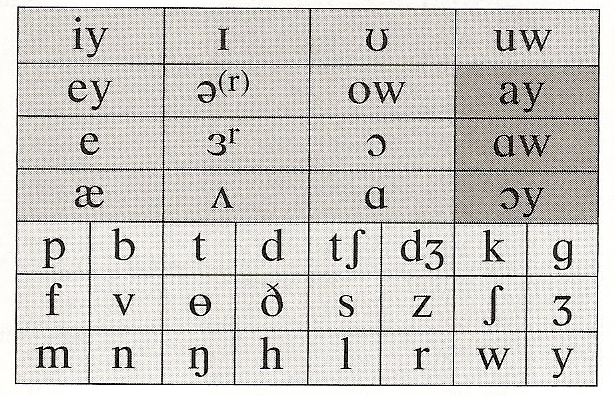
\includegraphics{images/nae-phonemes.jpg}
\caption{Phonemes in NAE\label{phonemic-chart}}
\end{figure}

To be able to use phonemes in software an ASCII representation is more
suitable. The standard for General American English is the
\emph{Arpabet}. Here each phoneme is mapped to one or two capital
letters. The digits \texttt{0}, \texttt{1} and \texttt{2} signify stress
markers: no stress, primary and secondary stress respectively.

\subsubsection{Phonetic dictionaries}\label{phonetic-dictionaries}

Phonetic dictionaries map words to one or more versions of phoneme
sequences.

A phonetic representation of a word is specified manually based on the
knowledge of how written words \emph{actually sound} when spoken.

An excerpt from the CMU EN-US Pronouncing Dictionary
(\emph{cmudict-en-us.dict}, \hyperref[ref-cmuDict]{2015}) looks like
this (phonemes are given in Arpabet representation):

\begin{verbatim}
...
abdollah AE B D AA L AH
abdomen AE B D OW M AH N
abdomen(2) AE B D AH M AH N
abdominal AE B D AA M AH N AH L
abdominal(2) AH B D AA M AH N AH L
...
\end{verbatim}

The dictionary has 133.425 entries. Generally only words that are in the
phonetic dictionary being used can be recognized during speech
recognition. \emph{Grapheme\footnote{A grapheme is ``the smallest unit
  used in describing the writing system of a language'' (Florian,
  \hyperref[ref-florian1996blackwell]{1996}). Some languages have strong
  correspondences between phonemes and graphemes, this is not a
  necessary relationship however -- the English word ``debt'' for
  example has the grapheme \texttt{\textless{}b\textgreater{}}, which is
  not represented by a corresponding sound.}-to-Phoneme converters}
(G2P) however make it possible to get phoneme sequence hypotheses for
arbitrary words (i.e arbitrary sequences of graphemes). While these
results are on average less accurate than manually created variants,
they play a vital role in texts with many technical terms as these are
often not included in phonetic dictionaries.

\subsubsection{Search}\label{search}

Search is the basic abstraction that lies at the center of the speech
recognition process, which is called the \emph{decoding phase}. The
recognition process is implemented as a search algorithm on a directed
search graph. This graph is constructed by taking different information
dimensions into account: typically an acoustic model, a language model
and phonetic dictionary. An example graph is shown in figure
\ref{graph}\footnote{The graph is taken from Walker et al.
  (\hyperref[ref-whitepaper]{2004}).}. Here words (from a language
model) are shown in rectangles, phonemes (from a phonetic dictionary) as
dark circles and audio input features as white circles (from an acoustic
model). The general search space topology and phonetic context size is
dependent on the specific algorithm used.

\begin{figure}[htbp]
\centering
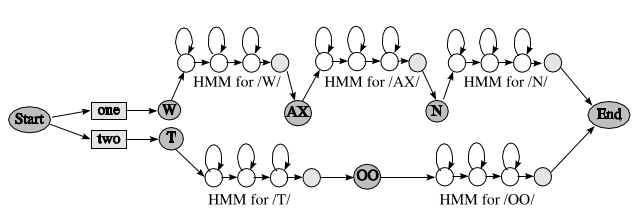
\includegraphics{images/graph.png}
\caption{Search graph with example words ``one'' and
``two''\label{graph}}
\end{figure}

\subsubsection{Acoustic models}\label{acoustic-models}

An acoustic model (AM) describes the relation between an audio signal
and the probability that this signal represents a given phoneme.

Acoustic models are created by \emph{training} them on a \emph{corpus}
of audio recordings and matching transcripts. When being used in the
context of speaker-independent recognition, these models are trained
with a variety of speakers that represent a broad spectrum of the
language/accent that the acoustic model should represent.

During the decoding phase the acoustic model and a phonetic dictionary
are used to match sequences of small audio ``slices'' to possible
phonemes and those phonemes to possible word sequence hypotheses.

However, acoustic models alone are not sufficient for speech recognition
as they do not have the ``higher-level'' linguistic information
necessary to distinguish e.g.~between homonyms and similar-sounding
phrases such as ``wreck a nice beach'' and ``recognize speech''
(Marquard, \hyperref[ref-marquard]{2012}, p. 11). This information is
provided by \emph{language models}.

\subsubsection{Language Models}\label{language-models}

Language models (LM) guide and constrain the search process that a
speech recognition system performs by assigning probabilities to
sequences of words. The basic premise, called Markov assumption, is that
the overall probability of a sentence with the words \(w_1,...,w_n\) can
be approximated as follows:

\[P(w_1,...,w_n) = \prod_{i=1}^m P(w_i \mid w_1,...w_{i-1})\]

This assumption says that an approximate probability of a given word can
be calculated only by looking at the last \emph{n} - 1 prior words. This
property significantly decreases statistical complexity and thus makes
it computationally feasible.

An example approximation with a bigram model for the sentence ``I saw
the red house'' represented as \(P(\text{I, saw, the, red, house})\)
would look like \[
  P(\text{I} \mid \langle s \rangle) \cdot
  P(\text{saw} \mid \text{I}) \cdot
  P(\text{the} \mid \text{saw}) \cdot
  P(\text{red} \mid \text{the}) \cdot
  P(\text{house} \mid \text{red}) \cdot
  P(\langle s \rangle \mid \text{house})
\]

The most commonly used form of language models are \emph{n-gram language
models}. In the context of a language model an \emph{n-gram} is a
sequence of \emph{n} words. 1-grams are called \emph{unigrams}, 2-grams
are called \emph{bigrams} and 3-grams are called \emph{trigrams}. An
\emph{n-gram language model} maps a set of \emph{n-grams} to
probabilities that they occur in a given piece of text.

N-gram language models do not need to be constrained to one type of
n-gram; the \emph{Generic US English Language Model}
(\emph{cmusphinx-5.0-en-us.lm}, \hyperref[ref-cmuLm]{2015}) from
CMUSphinx we will use as the baseline for our approach consists of 1-,
2, and 3-grams, for example.

Language models are trained by applying statistical methods on a text
corpus. Analogous to acoustic models, generic language models use huge
text corpora with a broad variety of topics. It is however possible to
train language models on small and specialized text corpora, which is
the central technical foundation for the approach discussed in this
thesis.

\subsection{Work done on ASR for lecture
transcription}\label{work-done-on-asr-for-lecture-transcription}

I will now give an overview over the scientific work done on lecture
transcription, using Marquard (\hyperref[ref-marquard]{2012}) as a
guiding reference.

The research for speech recognition on lectures can be partitioned into
two general approaches: generalization approaches and specialization
approaches.

\subsubsection{Generalization
approaches}\label{generalization-approaches}

Generalization approaches try to create models that capture common
characteristics of lectures. Those characteristics include highly
spontaneous presentation style and ``strong coarticulation effects,
non-grammatical constructions, hesitations, repetitions, and filled
pauses'' (Yamazaki, Iwano, Shinoda, Furui, \& Yokota,
\hyperref[ref-yamazaki]{2007}). Glass, Hazen, Hetherington, \& Wang
(\hyperref[ref-glass]{2004}) note the ``colloquial nature'' of lectures
as well as the ``poor planning at the sentence level {[}and{]} higher
structural levels''.

The generalization approach has been applied on the acoustic model
level: Cettolo, Brugnara, \& Federico (\hyperref[ref-cettolo]{2004})
have examined adapting a generic acoustic model to account for
spontaneous speech phenomena (``filler sounds'').

While a subfield of ASR called ``speaker diarization'' tries to account
for the interactivity between lecturers and students by identifying
multiple speakers, most research treats lectures as single speaker
events with the audience as background noise.

Generalization approaches at the language model level try to model
common linguistic traits of the lecture genre (this can be called the
\emph{macro level}). Kato, Nanjo, \& Kawahara
(\hyperref[ref-kato2000]{2000}) investigate topic-independent language
modeling by creating a large corpus of text from lecture transcripts and
panel discussions and then removing topic-specific keywords.\footnote{In
  a second step they combine this generalization technique with a
  specialization technique by adapting the resulting LM with a
  lecture-specific language model by using preprint papers of a given
  lecture.}

\subsubsection{Specialization
approaches}\label{specialization-approaches}

Specialization approaches try to use context specific to a single
lecture (\emph{meso level}) or parts of a single lecture (\emph{micro
level}\footnote{The three levels are taken from Marquard
  (\hyperref[ref-marquard]{2012}).}).

Methods used for creating LMs from context information can be
categorized into two approaches: direct usage of lecture slides and
notes for the creation of LMs versus usage of ``derived'' data from
these materials. Deriving data by using keywords found in slides, using
them as web search query terms and using the found documents as the
basis for LM creation is explored in Munteanu, Penn, \& Baecker
(\hyperref[ref-munteanu]{2007}), Kawahara, Nemoto, \& Akita
(\hyperref[ref-kawahara08]{2008}) and Marquard
(\hyperref[ref-marquard]{2012}).

Using the whole text from lecture slides has been explored by Yamazaki
et al. (\hyperref[ref-yamazaki]{2007}). They compare the meso level with
the micro level by dynamically adapting the LM to the speech
corresponding to a particular slide. Kawahara et al.
(\hyperref[ref-kawahara08]{2008}) also examine dynamic local
slide-by-slide adaption and compare it to global topic adaption using
Probabilistic Latent Semantic Analysis (PLSA)\footnote{Latent Semantic
  Analysis is an approach to document comparison and retrieval which
  relies on a numeric analysis of word frequency and proximity. } and
web text collection, concluding that the latter performs worse than the
former because of a ``worse orientation to topic words''.

\subsubsection{Conclusion }\label{conclusion}

Our approach can thus be classified as a specialization approach with
exclusive ``direct'' use of the lecture material. Specifically, it does
not try to extend the material corpus by using derived data; it neither
tries to consider the \emph{micro level}, which would imply to look at
parts of a single lecture.

After having located our approach against the backdrop of the different
approaches currently explored by the scientific community, I will now
continue to present the test data used.

\section{Test data}\label{data}

The test data I will use for evaluating our approach are from \emph{Open
Yale Courses}\footnote{\url{http://oyc.yale.edu/}}, which is a selection
of openly available lectures from Yale University. It consists of 42
courses from 25 departments. Each course has about 20-25 sessions that
have an average length of 50 minutes. Each lecture is provided with good
quality audio and video recordings, precise manual transcripts and
lecture material when available. Unfortunately only about 20\% of the
lectures have lecture notes or slides and most materials from the
natural and formal science departments (physics, astronomics,
mathematics) consist of hand-written notes, making them unsuitable for
our approach. All talks are in English.

I have chosen the following lectures: (Department, Course, Lecture
Number - Title, abbreviation)

\begin{itemize}
\item
  \emph{Biomedical Engineering}: Frontiers of Biomedical Engineering, 1
  - What is Biomedical Engineering? (\texttt{biomed-eng-1})
\item
  \emph{Environmental Studies}: Environmental Politics and Law, 8 -
  Chemically Dependent Agriculture (\texttt{environmental-8})
\item
  \emph{Geology \& Geophysics}: The atmosphere, the ocean, and
  environmental change, 8 - Horizontal transport (\texttt{geology-8})
\item
  \emph{Philosopy}: Philosophy and the science of human nature, 8 -
  Flourishing and Detachment (\texttt{human-nature-8})
\item
  \emph{Psychology}: Introduction to Psychology, 14 - What Motivates Us:
  Sex (\texttt{psy-14})
\item
  \emph{Psychology}: Introduction to Psychology, 5 - What Is It Like to
  Be a Baby: The Development of Thought (\texttt{psy-5})
\end{itemize}

The main selection criterion here was topical diversity, the challenge
being that the majority of talks with computer-parsable notes was from
the humanities.

\subsection{Material overview}\label{material-overview}

The available material is very heterogeneous. I will now give an
overview with excerpts which will serve as a basis for examining at a
later point if the quality and quantity of the supplied material is
correlated with the amount of improvement of our approach.

\texttt{geology-8} supplies a 2-page excercise sheet.

\begin{quote}
``Mars has a radius of 3.39 x \(10^6\) m and a surface gravity of 3.73
\(ms^{-2}\). Calculate the escape velocity for Mars and the typical
speed of a CO2 molecule (assume T = 250 K). How can Mars retain its CO2
atmosphere? (Hint: the molecular weight of carbon dioxide is 44. Use the
formulae given in class.) {[}\ldots{}{]}''
\end{quote}

\texttt{biomed-eng-1} provides a 7-page glossary of technical terms.

\begin{quote}
``{[}\ldots{}{]} active transport - the transport of molecules in an
energetically unfavorable direction across a membrane coupled to the
hydrolysis of ATP or other source of energy

ATP (adenosine 5'-triphosphate) - a nucleotide that is the most
important molecule for capturing and transferring free energy in cells.
Hydrolysis of each of the two high-energy phosphoanhydride bonds in ATP
is accompanied by a large free-energy change (``G) of 7 kcal/mole

aquaporin -- a water channel protein which allows water molecules to
cross the cell membrane much more rapidly than through the phospholipid
bilayer {[}\ldots{}{]}"
\end{quote}

\texttt{human-nature-8} provides reading assignments for four books with
short summaries each.

\begin{quote}
``{[}A{]} Epictetus, The Handbook

Background information about the Stoic philosopher Epictetus (c. 50-130
CE) and his famous work Encheiridion (The Handbook) appears in Nicholas
White's introduction to our translation. White has also added footnotes
that explain points of potential confusion.

As the title indicates, The Handbook is intended as a tidy introduction
to a more complex philosophical outlook. It is written in an accessible
and engaging style.

The Stoic movement originated around 300 BCE and flourished for over
five hundred years. The Stoics believed that the external world is
deterministic: its state at any time is completely determined by its
prior states. So, they maintained, it is pointless to wish for things to
be different because to do so is to wish for something impossible. A
wise person would, therefore, accept whatever befalls them without
desiring that things go otherwise -- hence the English word `stoic.'
\end{quote}

\begin{quote}
Passages to focus on/passages to skim

I encourage you to read the text in full, at a steady reading pace.
{[}\ldots{}{]}"
\end{quote}

\texttt{psy-14/5} and \texttt{enviromental-8} provide
\textasciitilde{}10-page slides with a typical amount of text.

\subsection{Conclusion}\label{conclusion-1}

Only about 20\% of the courses have lecture material at all; of these
only about 20\% actually have typical ``slides'' -- the rest provides
other heterogenous kinds of material. While it cannot be inferred from
this dataset that this is a general condition, it nevertheless shows a
clear ``real-world'' disadvantage of an approach necessarily relying on
lecture materials. We will look at the impact of the varying quality and
quantity in the analysis later on.

\section{The LM-Interpolation
approach}\label{the-lm-interpolation-approach}

I will now describe the LM-Interpolation approach. The high level
overview is as follows: we will use the open source speech recognition
framework Sphinx 4\footnote{Homepage:
  \url{http://cmusphinx.sourceforge.net/wiki/sphinx4:webhome}} as the
software for performing speech recognition. Sphinx 4 has a modular
architecture which allows specifying components of the whole process per
configuration. It provides multiple implementations of LMs\footnote{Overview:
  \url{http://cmusphinx.sourceforge.net/doc/sphinx4/edu/cmu/sphinx/linguist/language/ngram/LanguageModel.html}},
the default one being an n-gram model.

It also provides an \texttt{InterpolatedLanguageModel}\footnote{Javadoc:
  \url{http://cmusphinx.sourceforge.net/doc/sphinx4/edu/cmu/sphinx/linguist/language/ngram/InterpolatedLanguageModel.html}}
(ILM) which allows to specify multiple LMs and weights and to
interpolate the probabilities for a given n-gram from all models'
probabilities (\(p = w_1*p_1 + w_2*p_2 + \ldots\) where \(w_n\) are the
weights (\(\sum_{i=1}^n(w_i) = 1\)) and \(p_i\) is the probability for a
given n-gram in \(LM_i\)).

The purpose of the ILM in our approach is to factor in the importance of
keywords. These keywords have to be supplied in the form of an n-gram
language model. For this we extract text content from the lecture
material, preprocess it and create an n-gram LM from the resulting
corpus. Sphinx 4 is then run a) with a generic English n-gram LM only
and b) with the ILM configured to use the generic English LM and the
keyword language model in a specified weighting. Finally the two
resulting transcriptions are compared with a selection of metrics.

As an example, the 1-gram \emph{sex} has a probability of 2.82\% in the
keyword model of \texttt{psy-14}, but a probability of 0.012\% in the
generic English LM.\footnote{(\emph{cmusphinx-5.0-en-us.lm},
  \hyperref[ref-cmuLm]{2015})} When using interpolation with a 50/50
weighting, the result is
\(2.82\% \cdot 0.5 + 0.012\% \cdot 0.5 = 1.416\%\), which is an increase
by the factor \textasciitilde{}117 over the generic probability.

I will now give an overview over the Sphinx 4 architecture, followed by
a description of the implementation of the approach.

\subsection{Sphinx 4 architecture}\label{sphinx-4-architecture}

The overall architecture of Sphinx 4 as shown in figure \ref{sphinx4} is
comprised of three primary modules: the \emph{FrontEnd}, the
\emph{Decoder} and the \emph{Linguist}.\footnote{The following
  description is based on Walker et al.
  (\hyperref[ref-whitepaper]{2004}).} The \emph{FrontEnd} takes one or
more input signals and parameterizes them into a sequence of
\emph{Features}. The \emph{Linguist} takes any type of standard language
model, pronunciation information from a phonetic \emph{Dictionary} and
information from one or more sets of \emph{AcousticModels}, generating a
\emph{Search Graph}. The \emph{SearchManager} in the \emph{Decoder} uses
\emph{Features} from the \emph{FrontEnd} to perform decoding. Each of
the components (written in italics) are interfaces for which the actual
implementation can be configured at runtime.

\subsubsection{FrontEnd}\label{frontend}

The \emph{FrontEnd} parameterizes an \emph{Input} signal into a sequence
of output \emph{Features}. This process is realized as one or multiple
chains that can run in parallel, permitting simultaneous computation of
different types of parameters from the same or different input signals.

\subsubsection{Linguist}\label{linguist}

The \emph{Linguist} encapsulates the details of generating a
\emph{SearchGraph} used by the \emph{SearchManager} in the
\emph{Decoder}. It consists of the \emph{LanguageModel}, the
\emph{Dictionary} and the \emph{AcousticModel}.

\emph{LanguageModel} implementations can typically be categorized into
graph-driven grammars and n-gram models. The latter are primarily
differentiated by their usage parameters (e.g.~small vs.~very big LMs;
input formats).

\emph{Dictionary} provides the pronunciations for words found in the
\emph{LanguageModel}. A G2P Model can be specified in the configuration
which will statistically model missing entries in the dictionary.

The \emph{AcousticModel} provides a mapping between a phoneme and an HMM
that can be scored against incoming \emph{Features} provided by the
\emph{FrontEnd}, also taking word-contextual information into account.

\subsubsection{SearchGraph}\label{searchgraph}

The primary data structure in the decoding phase is the
\emph{SearchGraph}. It is a directed graph whose nodes are
\emph{SearchStates} that are either \emph{emitting} or
\emph{non-emitting}. \emph{Emitting} nodes can be scored against an
incoming acoustic feature, while \emph{non-emitting} nodes represent
higher-level linguistic constructs such as words and phonemes that are
not directly scored against these features.

\subsubsection{Decoder}\label{decoder}

The \emph{Decoder} uses \emph{Features} from the \emph{FrontEnd} by
using a \emph{SearchManager} that controls the \emph{Linguist's}
\emph{SearchGraph} to generate \emph{Result} hypotheses. The
\emph{Decoder} tells the \emph{SearchManager} to recognize a set of
\emph{Feature} frames. At each step, the \emph{SearchManager} creates a
\emph{Result} object that contains all paths that ``reached a final
non-emitting state''.

\begin{figure}[htbp]
\centering
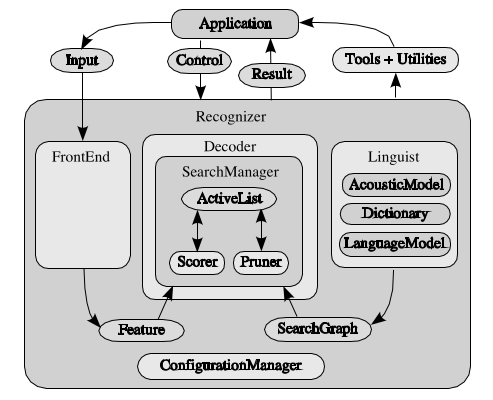
\includegraphics{images/sphinx4_150.png}
\caption{Sphinx 4 architecture \label{sphinx4}}
\end{figure}

\subsection{Implementation}\label{implementation}

The pipeline is implemented with a collection of standalone command line
tools and a set of shell and Python scripts\footnote{The source code is
  available here:
  \url{https://github.com/jonathanewerner/bachelor/tree/master/bin}}.

The tasks are the following, in chronological order:

\begin{enumerate}
\def\labelenumi{\arabic{enumi}.}
\item
  \textbf{Prepare the input}

  \begin{itemize}
  \tightlist
  \item
    The audio file is converted into Sphinx 4 compatible format (16khz,
    16bit mono little-endian).
  \item
    A testcase folder with a given shortname (e.g. \texttt{psy-15}) is
    created in the \texttt{results}-directory\footnote{\url{https://github.com/jonathanewerner/bachelor/tree/master/results}}
    of the source code repository.
  \item
    The reference transcript, the material (PDF format is required) and
    the converted audio file are moved into a \texttt{resources}
    subfolder of the testcase folder.
  \end{itemize}
\item
  \textbf{Create a keyword LM from lecture material}

  \begin{itemize}
  \tightlist
  \item
    \texttt{pdftohtml\ -i\ -xml} is applied on the given material PDF.
    The XML output representation then becomes the input for
    \texttt{pdfreflow}\footnote{pdftohtml
      (\url{http://pdftohtml.sourceforge.net/}) and pdfreflow
      (\url{http://sourceforge.net/projects/pdfreflow/}) are open source
      linux command line utilities}. Compared to the tool
    \texttt{pdftotext} the combination of these 2 tools preserves
    paragraphs correctly, whereas \texttt{pdftotext} represents each
    line break in the input PDF as a new paragraph in the output text
    file. This is a significant disadvantage for the LM creation step,
    as in this case a newline in the input file constitutes the semantic
    ``end of sentence'' -- so that a sentence split into 4 lines by
    \texttt{pdftotext} would count as 4 sentences in the LM.
  \item
    The HTML output from \texttt{pdfreflow} is filtered by taking only
    relevant HTML-tags such as \texttt{\textless{}p\textgreater{}}'s
    (paragraphs) and \texttt{\textless{}blockquote\textgreater{}}'s,
    further improving the content-to-noise ratio.
  \item
    The resulting text is then preprocessed for optimal compatibility
    with the LM creation tool by removing punctuation and superfluous
    whitespace\footnote{I use a combination of command line text
      processing (sed) and a perl script from Stephen Marquard here.}.
  \item
    The resulting corpus then becomes the input for
    \texttt{estimate-ngram}, an LM creation tool from the MIT Language
    Modeling Toolkit\footnote{\url{https://code.google.com/p/mitlm/wiki/EstimateNgram}}
    (MITLMT).
  \end{itemize}

  For clarification intermediate results from this step follow as an
  example. They are taken from the test case \texttt{psy-5}\footnote{``Introduction
    to Psychology, 5 - What Is It Like to Be a Baby: The Development of
    Thought''}. Figure \ref{slide} shows an example slide.

  \begin{figure}[htbp]
  \centering
  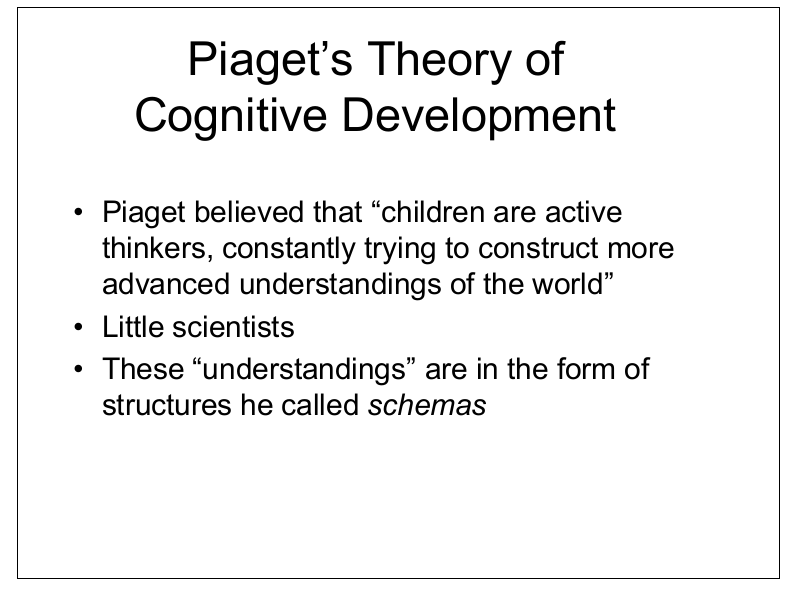
\includegraphics{images/slide_250.png}
  \caption{Slide from lecture \texttt{psy-5} \label{slide}}
  \end{figure}

  When using \texttt{pdftotext} the result for the given slide is as
  follows:

\begin{verbatim}
Piaget’s Theory of
Cognitive Development
• Piaget believed that “children are active
thinkers, constantly trying to construct more
advanced understandings of the world”
• Little scientists
• These “understandings” are in the form of
structures he called schemas
\end{verbatim}

  Notice how each newline in the slide maps to a newline in the output.
  When using the combination of \texttt{pdftohtml} and
  \texttt{pdfreflow} the result looks like this:

\begin{verbatim}
<p class="p9">Piaget’s Theory of
Cognitive Development </p>
<p class="p10">•  Piaget believed that “children are active
thinkers, constantly trying to construct more
advanced understandings of the world” </p>
<blockquote class="b9">•  Little scientists </blockquote>
<p class="p10">•  These “understandings” are in the form of
structures he called <i>schemas</i> </p>
\end{verbatim}

  Notice how a paragraph is captured in a
  \texttt{\textless{}p\textgreater{}}-tag. This allows to extract a
  sentence as one line in the corpus. After applying the preprocessing
  described above the final corpus for the slide looks like this (where
  ``..'' marks a line continuation):

\begin{verbatim}
piagets theory of cognitive development
piaget believed that children are active thinkers constantly
.. trying to construct more advanced understandings of the world
little scientists
these understandings are in the form of structures he called schemas
\end{verbatim}
\item
  \textbf{Convert transcript to reference corpus}

  The transcript from Open Yale is supplied as HTML. We apply processing
  steps to transform it to a corpus ready to be consumed by the analysis
  tool (no punctuation, all lowercase). As these are just specific to
  the format chosen by Open Yale Courses, the details are omitted, as
  they are of no general relevance.
\item
  \textbf{Run Sphinx 4 in baseline and interpolated mode}

  \texttt{bin/sphinx-interpolated.py}\footnote{\url{https://github.com/jonathanewerner/bachelor/blob/master/bin/sphinx-interpolated.py}}
  supplies a wrapper for interfacing with Sphinx 4. The Java API of
  Sphinx 4 is exposed for command line usage by a JAR package which
  bundles the Sphinx 4 libraries and a small \texttt{Main} class. This
  class uses command line arguments supplied by
  \texttt{bin/sphinx-interpolated.py} to correctly configure Sphinx 4
  and start the actual recognition.

  Each testcase folder has a configuration file which specifies the
  models to be used by the test run:

\begin{verbatim}
  {
    "acousticModelPath": "en-new/cmusphinx-en-us-5.2",
    "dictionaryPath": "en-new/cmudict-en-us.dict",

    "languageModelPath": "en-new/cmusphinx-5.0-en-us.lm",
    "keywordModelPath": "model.lm",
    "g2pModelPath": "en-new/en_us_nostress/model.fst.ser",

    "resultsFolder": "biomed-eng-1"
  }
\end{verbatim}

  \texttt{bin/sphinx-interpolated.py} interprets the ``global'' models
  relative to the repository root folder \texttt{models}, the
  \texttt{resultsFolder} relative to the root folder \texttt{results}
  and the \texttt{keywordModelPath} relative to the
  \texttt{resultsFolder}. It then supplies the absolute paths to the
  JAR. It also supplies absolute output file paths for the transcription
  result and transcription word timing results.

  This setup ensures reproducible results, as the environment of a given
  testcase is exactly specified (as long as the same binaries and script
  versions are assumed).

  \texttt{bin/sphinx-interpolated.py} can now be used to run the
  baseline and/or interpolated version.
\item
  \textbf{Analyze and compare the results}

  Finally the results from the two recognition runs are analyzed and
  compared by running
  \texttt{bin/hotword-analyze\ \textless{}testcase\ folder\ name\textgreater{}}.
  This does two things: a) run comparison and metrics generation and b)
  keyword visualization.

  5.1 \emph{Run comparison and metrics generation}

  This first calls \texttt{bin/wer.py}\footnote{\texttt{wer.py} has been
    adapted from
    \url{http://progfruits.blogspot.de/2014/02/word-error-rate-wer-and-word.html}}
  on each run, which will calculate the WER and show a summary of
  substituted (SUB), inserted (INS) and deleted (DEL) words when
  comparing the reference (REF) to the hypothesis (HYP):

\begin{verbatim}
OP  | REF     | HYP
INS | ****    | this
INS | ****    | is
INS | ****    | that
OK  | this    | this
OK  | is      | is
OK  | a       | a
OK  | course  | course
SUB | a       | that
SUB | version | aversion
OK  | of      | of
OK  | which   | which
SUB | i've    | i
OK  | taught  | taught
INS | ****    | him
...
...
{'Sub': 1230, 'Ins': 674, 'WER': 0.316, 'Del': 324, 'Cor': 5492}
\end{verbatim}

  In a second step it compares the two WER result files with
  \texttt{bin/compare-wer.py}.

  The result is an HTML file which shows a) a comparison table with the
  columns \emph{reference word}, \emph{baseline hypothesis} and
  \emph{interpolated hypothesis} and b) various statistical measures
  which will be explored later. The table (shown in Figure
  \ref{wer-comparison}) represents correctly recognized words in green
  color and incorrect words in red. It also marks words that have been
  improved in the interpolated version with a green border and words
  that have been worsened with a red border.

  \begin{figure}[htbp]
  \centering
  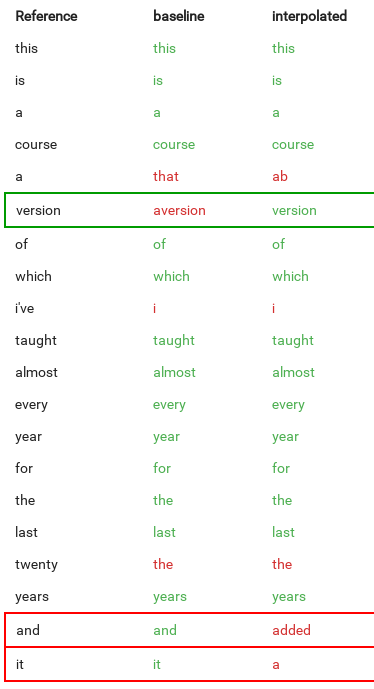
\includegraphics{images/wer-comparison_150.png}
  \caption{WER comparison\label{wer-comparison}}
  \end{figure}

  5.2 \emph{Keyword visualization}

  Data from the reference and the recognition results is compiled into a
  format suitable for consumption by a visualization module, which will
  be discussed in chapter \ref{viz}.
\end{enumerate}

All intermediate steps from the pipeline are represented as files in the
testcase folder. Table \ref{files} gives an overview of the files
created by each pipeline step.

\begin{longtable}[c]{@{}ll@{}}
\caption{File results of a testcase run\label{files}}\tabularnewline
\toprule
File & Description\tabularnewline
\midrule
\endfirsthead
\toprule
File & Description\tabularnewline
\midrule
\endhead
\textbf{Step 1: Prepare the input} &\tabularnewline
\texttt{resources/audio.mp3} & original audio\tabularnewline
\texttt{resources/audio.wav} & converted audio\tabularnewline
\texttt{resources/slides.pdf} & lecture material\tabularnewline
\texttt{resources/transcript.html} & lecture transcript\tabularnewline
\texttt{config.json} & run configuration\tabularnewline
&\tabularnewline
\textbf{Step 2: Create a keyword LM} &\tabularnewline
\texttt{slides.corpus.txt} & lecture material corpus\tabularnewline
\texttt{model.lm} & keyword LM\tabularnewline
&\tabularnewline
\textbf{Step 3: Convert reference to corpus} &\tabularnewline
\texttt{reference.corpus.txt} & reference transcription
corpus\tabularnewline
\texttt{reference\_wordcounts.json} & reference transcription word
counts\footnote{They are needed for the visualization later.}\tabularnewline
&\tabularnewline
\textbf{Step 4: Run Sphinx 4} &\tabularnewline
\texttt{sphinx\_log\_baseline.txt} & Sphinx 4 logging
output\tabularnewline
\texttt{sphinx\_log\_interpolated.txt} &\tabularnewline
\texttt{sphinx\_result\_baseline.txt} & Sphinx 4
transcription\tabularnewline
\texttt{sphinx\_result\_interpolated.txt} &\tabularnewline
\texttt{sphinx\_word\_times\_baseline.txt} & Sphinx 4 word
times\tabularnewline
\texttt{sphinx\_word\_times\_interpolated.txt} &\tabularnewline
&\tabularnewline
\textbf{Step 5.1: WER comparison / metrics generation} &\tabularnewline
\texttt{results.json} & run metrics in json format\footnote{This eases
  parsability for aggregating multiple testcase results later.}\tabularnewline
\texttt{wer\_baseline.txt} & WER table / metrics\tabularnewline
\texttt{wer\_interpolated.txt} &\tabularnewline
\texttt{wer\_comparison.html} & rich WER comparison +
metrics\tabularnewline
&\tabularnewline
\textbf{Step 5.2: Keyword visualization} &\tabularnewline
\texttt{cloud\_baseline.json} & data representation for
visualization\tabularnewline
\texttt{cloud\_interpolated.json} &\tabularnewline
\bottomrule
\end{longtable}

\section{Analysis}\label{analysis}

I will now discuss how to evaluate the usefulness of the
LM-Interpolation approach in light of the goal to improve recognition
accuracy of interesting keywords.

\subsection{Approaching a good metric}\label{approaching-a-good-metric}

We want to find a metric that describes if and how much the interpolated
version improves upon the baseline version. The ``canonical'' metric
used to evaluate speech recognition performance is called \emph{Word
Error Rate} (WER). The WER is derived from taking the Levenstein
distance at the word level between a reference transcript and the
recognition result. WER is calculated as:

\[ WER = \frac{S + D + I}{N} \]

where

\begin{itemize}
\tightlist
\item
  \(S\) is the number of substitutions
\item
  \(D\) is the number of deletions
\item
  \(I\) is the number of insertions
\item
  \(N\) is the number of words in the reference (\(N = S+D+C\), where
  \(C\) is the number of correct words)
\end{itemize}

This approach circumvents the problem that the reference and the
recognition result get ``out of sync'' when words are inserted or
removed.

The problem of using WER for our purposes is twofold: 1. It does not
help to answer the question of how much our approach improves the
accuracy of keywords; it only pertains to \emph{all} words. 2. It
penalizes \emph{insertions}. But insertions are not relevant to the
question of how many of the keywords from the reference transcript have
been detected. Insertions only matter when we are interested in the
\emph{sentence integrity} of the result transcript. In our case, we do
not care if there are superfluous words \emph{between} correctly
recognized keywords\footnote{Although there might be cases of technical
  terms that are compound words -- in that case an insertion in between
  the compound word would be problematic. Detection of this edge case is
  however beyond the scope of our approach.}.

These considerations lead to the conclusion that a first improvement
over regular \emph{WER} would be to just look at the \emph{detection
rate} of words, where detection rate describes the proportion of words
from a transcript that have been correctly recognized. This can be
expressed by using WER in a first step in order to get the benefit of
word synchronization and then filtering out insertions in a second step.
It is not necessary to filter out deletions as these can be interpreted
as non-detected words.

A further improvement consists in just considering the words which are
part of the material corpus. By just taking the words that we used to
create the material corpus for our interpolated LM we can precisely
evaluate the improvement effect of this change. However, this is still
not perfect. The lecture material corpus includes a substantial amount
of words that would not be classified as ``keywords'': filler words and
very common words. One approach to sort them out is subtracting a set of
top \(x\) most common words (\emph{\(top_X\) words}) from this list. The
resulting metric can then be parameterized on the given \(x\). This is
an idea that Marquard uses when he proposes the metric ``Ranked Word
Correct Rate'' (RWCR-n):

\begin{quote}
``RWCR-n is defined as the Word Correct Rate for all words in the
document which are not found in the first n words in a given general
English word dictionary with words ranked from most to least frequent.''
(Marquard, \hyperref[ref-marquard]{2012}, p. 71)
\end{quote}

\subsubsection{Lemmas}\label{lemmas}

When searching for a specific term the user is interested in the
\emph{lemma}\footnote{A lemma, also called ``headword'', is the
  canonical form of a word that is chosen by convention to represent a
  group of lexemes that refer to the same meaning. A typical use would
  be the key of a dictionary entry.} for a given word: when he wants to
find occurences of ``child'' in the given lecture, occurences of
``children'' would also be relevant. This implies two things: 1) when
looking at the ``atomic'' level of improvements and degradations it is
more relevant to have lemmas as atoms and not words; and 2) the exact
matching (a hypothesis word is only ``correct'' if it exactly matches
the reference word) should be ``loosened'' to also mark hypothesis words
as correct if their lemmatized version matches the reference.

The same principle holds for the \(top_X\) words: we only want to
capture words for which the \emph{lemma} is not in the \(top_X\) words.

\subsubsection{Definition of KWDR-x and
WDR}\label{definition-of-kwdr-x-and-wdr}

We can distill these concerns into a definition of a metric called
\emph{Key Word Detection Rate} (\emph{KWDR-x}) where a keyword is
defined as the lemma of a word occuring in a given lemmatized lecture
material corpus, given that this lemma is not present in the \(top_X\)
list of most common words of the given language. A keyword is
\emph{detected} when it is \emph{lemma-equal}\footnote{Two words are
  defined as \emph{lemma-equal} when their lemmatized versions are
  equal. The words ``children'' and ``child'' are lemma-equal.} to the
corresponding word in the reference; if it has been substituted or
deleted, it is \emph{not detected}.

The \emph{Word Detection Rate} (\emph{WDR}) is analogously defined as
the rate of detected words, where a word is \emph{detected} when it is
lemma-equal to its reference.

The value of \(x\) has to be determined empirically: how many of the
\(top_X\) words should be filtered out? There has to be a balance
between not accidentally excluding keywords (i.e ``sex'' is in the
\(top_{500}\) words, but is a central keyword in lecture
\texttt{psy-14}) and filtering out enough filler words.

After experimenting with some values I chose \(x=500\) for my
measurements. It is hard to find a less ad hoc approach to determine the
``best'' \(x\), as there is no ``meta''-metric that would assess how
well a given \(x\) captures the goal of accurately describing the
detection accuracy of keywords; it necessarily is a ``best guess''.
\(x=500\) was chosen by looking at the relationship of \(x\) to
\(\Delta KWDR\) (the improvement in KWDR-500) in an example lecture, as
shown in figure \ref{x-to-KWDR}. For values of \(x\) below
\textasciitilde{}200 the growth of improvement is explained by the
gradual removal of filler words from the set of keywords. The
recognition accuracy of filler words is not improved by our approach
which is why they prevent the accuracy improvement of actual keywords to
be visible. Above \textasciitilde{}200 this factor is ruled out and the
chosen \(x\) value has only miniscule influence on the resulting KWDR.

\begin{figure}[htbp]
\centering
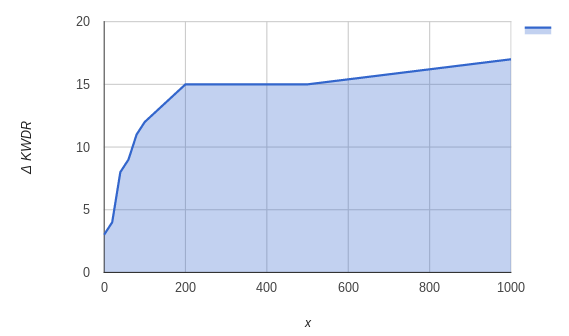
\includegraphics{images/kwdr_150.png}
\caption{Relation of x to \(\Delta KWDR\), compiled by running the
analysis on lecture \texttt{geology-8} with the x-values 0, 20, 40, 60,
80, 100, 200, 300, 400, 500 and 1000.\label{x-to-KWDR}}
\end{figure}

This strategy, while depending on choosing an ``ad hoc'' value, was
sufficient to validate our approach because it was possible to manually
evaluate the metric's ``precision'' by observing the resulting word
sets. Another approach would have been to take the \emph{tf-idf} (Term
Frequency - Inverse Document Frequency) as a criterion for
``keyword-ness'' of words. \emph{tf-idf} computes the ``relevance'' of a
word in the context of a document by taking into account the occurences
of the word in the document offset by the word's frequency in a broader
corpus. This way common words are rated lower although they occur
frequently in the given document. As such there is no need for the
arbitrary aspect of choosing a value of \(x\) and the negative side
effect of accidentally excluding a keyword. On the other hand there
would be the need to choose a threshold \emph{tf-idf} score which would
have to be reached for inclusion into the keyword set.

\subsubsection{Metrics overview}\label{metrics-overview}

The following metrics are evaluated, including secondary or derived
metrics:

\begin{itemize}
\tightlist
\item
  \(W\): Number of words
\item
  \(KW\): Number of keywords
\item
  \(WER_{A|B}\): Word Error Rate of baseline (A) / interpolated version
  (B)
\item
  \(WDR_{A|B}\): Word Detection Rate of baseline (A) / interpolated
  version (B)
\item
  \(KWDR_{A|B}\): KWDR = KWDR-500 for brevity = Keyword Detection Rate
  with \(x=500\) of baseline (A) / interpolated version (B)
\item
  \(W_{worse|improved}\): Proportion of worsened/improved words
\item
  \(KW_{worse|improved}\): Proportion of worsened/improved keywords
\item
  \(W_{worse|improved}(K)\): Proportion of worsened/improved words that
  are keywords
\item
  \(E\): \(W_{improved}(K) - W_{worse}(K)\): A percentage score for
  ``effectiveness'' of version B
\end{itemize}

\subsubsection{Example calculation}\label{example-calculation}

The use of all metrics can be exemplarily demonstrated on the lecture
\texttt{human-nature-8}: The lecture has 5342 words overall, of which
333 are keywords. When looking at the general WDR, run A and B both have
a score of 58\%. This can be ``split up'' by looking at
\(W_{worse|improved}\), which is 4\% each, meaning that 4\% (223/5342)
of the words have been improved from run A to B, but 4\% (221/5342) of
them have been worsened, which sums up to 0\% difference in WDR.

Secondly, the KWDR of A is 47\% (156/333 keywords) versus 62\% for B
(212/333 keywords). This improvement of 15\% can analogously be
explained by looking at \(KW_{worse|improved}\): when looking at the 333
keywords, 2\% (7/333) of them have been worsened, while 17\% (58/333)
have been improved. \(17-2 = 15\%\) explains the improvement from 47\%
to 62\%.

The last metric of \(W_{worse|improved}(K)\) looks at the overall
worsened/improved words and informs about the proportion of words that
were keywords. As mentioned, \(W_{worse}\) is 4\% (221 of the overall
5342 words have been worsened). What is the proportion of keywords in
this number? Analogously, what is the proportion of keywords when
looking at the overall improved words? This metric is key in identifying
the \emph{effectiveness} (E) of our approach: the \(W_{improved}(K)\)
value answers the question of how well our approach is targeted towards
improving the words we are interested in, the \(W_{worse}(K)\) value
answers the question of how big the ``side effect'' of worsening
keywords is. In the example \(W_{worse}(K)\) is 3\% (7/221) and
\(W_{improved}(K)\) is 26\% (58/223). This is great: of the 221 overall
worsened words only \textbf{7} were relevant in light of our goals. In
essence, we can interpret \(W_{improved}(K) - W_{worse}(K)\) as an
\textbf{effectiveness score}. We can say that our example has an
effectiveness of \(26-3=23\%\). An effectiveness of 100\% would mean
that \emph{all} words that were improved had been keywords and
\emph{none} of the worsened words had been keywords.

\subsection{Implementation of measurements
calculation}\label{implementation-of-measurements-calculation}

Measurements are calculated automatically by \texttt{bin/wer.py} and
\texttt{bin/compare-wer.py}. I will now outline some relevant
implementation details.

\texttt{bin/wer.py} performs a typical WER calculation algorithm. This
is run on version A (baseline) and B (interpolated). The results become
the input for \texttt{bin/compare-wer.py}. The \(top_{500}\) words are
taken from the \emph{Corpus of Contemporary American English}\footnote{\url{http://www.wordfrequency.info/free.asp}}.
The lemmatization of words is done by the \texttt{lemmatize} function of
\texttt{nltk.stem.wordnet.WordNetLemmatize}.

The KWDR of A and B is then calculated by iterating over both WER
results with insertions filtered out.

Each iteration operates on a tuple of (reference word, hypothesis A,
hypothesis B).

\begin{enumerate}
\def\labelenumi{\arabic{enumi}.}
\item
  For both hypotheses it checks if the reference word is
  \emph{lemma-equal} to the hypothesis word; if that is not the case,
  the reference word is put in a ``wrong words'' bin (one bin for A and
  B each).
\item
  If both hypotheses are correct, the next iteration is performed.
\item
  Else: if A is correct and B is wrong, the reference is put into the
  ``worsened'' bin; the other way, round it is put into the ``improved''
  bin.
\item
  Finally, if a hypothesis is wrong \emph{and} it is a keyword\footnote{It
    is a keyword if its lemma is in the lemmatized, \(top_x\)-words
    excluded material corpus.}, the reference is put into the ``wrong
  keyword'' bin (also one for each run).
\end{enumerate}

After the iterations are finished, the mentioned metrics are calculated
by simple calculation of the proportions, taking into account the size
of the resulting bins and overall measurements (like reference word
count).

As side effects, the bin contents as well as the calculated metrics are
exported to HTML and JSON for further manual inspection resp. result
aggregation.

\subsubsection{Example}\label{example}

The steps of this process can be made clearer by running through a small
example. The following toy data set serves as input:

\begin{itemize}
\item
  Material corpus: {[}axons the people psychology is
  rewarding{]}\footnote{Imagine this being taken from sparse slides with
    bullet points.}
\item
  Reference transcript: ``Axons are firing to stimulate people's
  minds.'' (This gets preprocessed to ``axons are firing to stimulate
  peoples minds'' in a previous step.)
\item
  \(Top_x\) words: {[}i are it is the people people's{]}
\item
  The WER results for A:

\begin{verbatim}
OP  | REF       | HYP
sub | axons     | accent
ok  | are       | are
ins | ****      | very
sub | firing    | tiring
ok  | to        | to
ok  | stimulate | stimulate
sub | peoples   | people
ok  | minds     | minds
{'Ins': 1, 'Cor': 4, 'WER': 0.571, 'Del': 0, 'Sub': 3}
\end{verbatim}
\item
  The WER results for B:

\begin{verbatim}
OP  | REF       | HYP
sub | axons     | axon
ok  | are       | are
ins | ****      | very
sub | firing    | tiring
ok  | to        | to
ok  | stimulate | stimulate
sub | peoples   | people
sub | minds     | may
{'Sub': 4, 'Ins': 1, 'Del': 0, 'Cor': 3, 'WER': 0.714}
\end{verbatim}
\end{itemize}

The inputs are transformed to the following forms (removed words
displayed as ``\textbf{-removed}''; changed words as \textbf{-old
+new}):

\begin{itemize}
\tightlist
\item
  Lemmatized material corpus: {[}\textbf{+axon} \textbf{-axons} the
  people psychology is rewarding{]}
\item
  Lemmatized \(top_x\) words: {[}i are it is the people
  \textbf{-people's}{]}
\item
  Lemmatized material corpus minus lemmatized \(top_x\) words
  (``keywords''): {[}axon \textbf{-the} \textbf{-people} psychology
  \textbf{-is} rewarding{]}
\end{itemize}

For the demonstration the following pseudo code conventions and
abbreviations are used:

\begin{itemize}
\tightlist
\item
  (a, b, c) = (1, 2, 3) is a destructuring assignment, binding a to 1, b
  to 2, c to 3
\item
  \texttt{ref} refers to the reference word, \texttt{hypA\textbar{}B} to
  the hypothesis from version A/B
\item
  l(word) refers to the lemmatized version of a given word
\item
  \texttt{-\textgreater{}} is equivalent to ``thus''
\item
  bin names:

  \begin{itemize}
  \tightlist
  \item
    wrong words from run X: \texttt{wrongX}
  \item
    wrong keywords from run A: \texttt{wrongKW\_X}
  \end{itemize}
\end{itemize}

The KWDR algorithm performs with the following intermediate steps:

\begin{itemize}
\tightlist
\item
  \textbf{Step 0}: (\texttt{ref}, \texttt{hypA}, \texttt{hypB}) =
  (axons, accent, axon)

  \begin{itemize}
  \tightlist
  \item
    l(\texttt{ref}) != l(\texttt{hypA}) -\textgreater{} add \texttt{ref}
    to \texttt{wrongA}
  \item
    l(\texttt{ref}) == l(\texttt{hypB}) -\textgreater{} do nothing
    (explanation: axon == axon)
  \item
    \texttt{hypA} was wrong, \texttt{hypB} was correct -\textgreater{}
    add \texttt{hypB} to \texttt{improved}
  \item
    \texttt{hypA} was wrong and a keyword -\textgreater{} add
    \texttt{ref} to \texttt{wrongKW\_A}
  \item
    \texttt{wrongA}: \texttt{{[}axons{]}}
  \item
    \texttt{wrongB}: \texttt{{[}\ {]}}
  \item
    \texttt{wrongKW\_A}: \texttt{{[}axons{]}}
  \item
    \texttt{wrongKW\_B}: \texttt{{[}\ {]}}
  \item
    \texttt{improved}: \texttt{{[}axons{]}}
  \item
    \texttt{worsened}: \texttt{{[}\ {]}}
  \end{itemize}
\item
  \textbf{Step 1}: (\texttt{ref}, \texttt{hypA}, \texttt{hypB}) = (are,
  are, are)

  \begin{itemize}
  \tightlist
  \item
    l(\texttt{ref}) == l(\texttt{hypA}) -\textgreater{} do nothing
  \item
    l(\texttt{ref}) == l(\texttt{hypB}) -\textgreater{} do nothing
  \item
    both are correct -\textgreater{} next iteration
  \end{itemize}
\item
  \textbf{Step 2}: (\texttt{ref}, \texttt{hypA}, \texttt{hypB}) =
  (firing, tiring, tiring)\footnote{Notice how the inserted row (marked
    with ``INS'' in the WER output) has been skipped).}

  \begin{itemize}
  \tightlist
  \item
    l(\texttt{ref}) != l(\texttt{hypA}) -\textgreater{} add \texttt{ref}
    to \texttt{wrongA}
  \item
    l(\texttt{ref}) != l(\texttt{hypA}) -\textgreater{} add \texttt{ref}
    to \texttt{wrongB}
  \item
    \texttt{wrongA}: \texttt{{[}axons,\ firing{]}}
  \item
    \texttt{wrongB}: \texttt{{[}firing{]}}
  \item
    \texttt{wrongKW\_A}: \texttt{{[}axons{]}}
  \item
    \texttt{wrongKW\_B}: \texttt{{[}\ {]}}
  \item
    \texttt{improved}: \texttt{{[}axons{]}}
  \item
    \texttt{worsened}: \texttt{{[}\ {]}}
  \end{itemize}
\item
  \textbf{Step 3/4}: (\texttt{ref}, \texttt{hypA}, \texttt{hypB}) = (to,
  to, to) / (stimulate, stimulate, stimulate)

  \begin{itemize}
  \tightlist
  \item
    l(\texttt{ref}) == l(\texttt{hypA}) -\textgreater{} do nothing
  \item
    l(\texttt{ref}) == l(\texttt{hypB}) -\textgreater{} do nothing
  \item
    both are correct -\textgreater{} next iteration
  \end{itemize}
\item
  \textbf{Step 5}: (\texttt{ref}, \texttt{hypA}, \texttt{hypB}) =
  (peoples, people, people)

  \begin{itemize}
  \tightlist
  \item
    l(\texttt{ref}) == l(\texttt{hypA}) -\textgreater{} do nothing
    (explanation: people == people)
  \item
    l(\texttt{ref}) == l(\texttt{hypB}) -\textgreater{} do nothing (same
    explanation)
  \item
    both are correct -\textgreater{} next iteration
  \end{itemize}
\item
  \textbf{Step 6}: (\texttt{ref}, \texttt{hypA}, \texttt{hypB}) =
  (minds, minds, may)

  \begin{itemize}
  \tightlist
  \item
    l(\texttt{ref}) == l(\texttt{hypA}) -\textgreater{} do nothing
  \item
    l(\texttt{ref}) == l(\texttt{hypB}) -\textgreater{} add \texttt{ref}
    to \texttt{wrongB}
  \item
    \texttt{wrongA}: \texttt{{[}axons,\ firing{]}}
  \item
    \texttt{wrongB}: \texttt{{[}firing,\ minds{]}}
  \item
    \texttt{wrongKW\_A}: \texttt{{[}axons{]}}
  \item
    \texttt{wrongKW\_B}: \texttt{{[}\ {]}}
  \item
    \texttt{improved}: \texttt{{[}axons{]}}
  \item
    \texttt{worsened}: \texttt{{[}minds{]}}
  \end{itemize}
\end{itemize}

\textbf{Results:}

\begin{itemize}
\tightlist
\item
  \texttt{wrongA}: \texttt{{[}axons,\ firing{]}}
\item
  \texttt{wrongB}: \texttt{{[}firing,\ minds{]}}
\item
  \texttt{wrongKW\_A}: \texttt{{[}axons{]}}
\item
  \texttt{wrongKW\_B}: \texttt{{[}\ {]}}
\item
  \texttt{improved}: \texttt{{[}axons{]}}
\item
  \texttt{worsened}: \texttt{{[}minds{]}}
\end{itemize}

\textbf{General/derived metrics:}

\begin{itemize}
\tightlist
\item
  \(W\) (count of words in reference): 7 (``axons are firing to
  stimulate peoples minds'')
\item
  \(KW\) (count of keywords in reference): 1 ({[}axon{]})
\item
  \texttt{worsenedKW}: all from \texttt{worsened} where the word is in
  KW -\textgreater{} \texttt{{[}\ {]}}
\item
  \texttt{improvedKW}: all from \texttt{improved} where the word is in
  KW -\textgreater{} \texttt{{[}axons{]}}
\end{itemize}

With these results we can calculate all metrics:

\begin{itemize}
\tightlist
\item
  \(WDR_A\) = \(1 - \frac{|wrongA|}{W} = 1 - \frac{2}{7} = ~71\%\)
\item
  \(WDR_B\) = \(1 - \frac{|wrongB|}{W} = 1 - \frac{2}{7} = ~71\%\)
\item
  \(W_{improved} = \frac{|improved|}{W} = \frac{1}{7} = ~14\%\)
\item
  \(W_{worsened} = \frac{|worsened|}{W} = \frac{1}{7} = ~14\%\)
\item
  \(KWDR_A\) = \(1 - \frac{|wrongKW_A|}{KW} = 1 - \frac{1}{1} = 0\%\)
\item
  \(KWDR_B\) = \(1 - \frac{|wrongKW_B|}{KW} = 1 - \frac{0}{1} = 100\%\)
\item
  \(KW_{improved} = \frac{|improvedKW|}{KW} = \frac{1}{1} = 100\%\)
\item
  \(KW_{worsened} = \frac{|worsenedKW|}{KW} = \frac{0}{1} = 0\%\)
\item
  \(W_{improved}(K) = \frac{|improvedKW|}{|improved|} = \frac{1}{1} = 100\%\)
\item
  \(W_{worsened}(K) = \frac{|worsenedKW|}{|worsened|} = \frac{0}{1} = 0\%\)
\item
  \(E = KW_{improved}(K) - KW_{worsened}(K) = 100\%\)
\end{itemize}

These metrics are more accessible when we look at the HTML output from
\texttt{compare-wer.py} as shown in figure \ref{viz-html-words}.

\begin{figure}[H]
\label{viz-html-words}
\centering
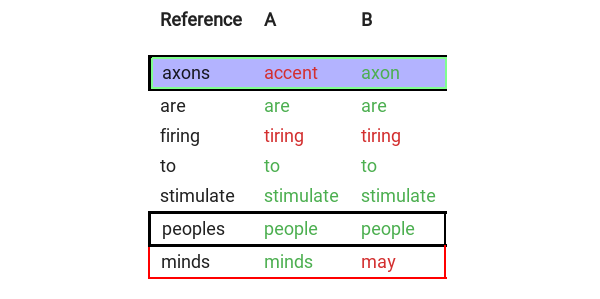
\includegraphics{images/analysis_150.png}
\caption{Visualization. Blue background: keyword. Green border: improved word. Red border: worsened word. Black border: lemmatization has changed a word.}
\end{figure}

\subsection{LM interpolation
weighting}\label{lm-interpolation-weighting}

It has been mentioned above that the weighting between the generic and
material LM can be specified. I experimented with different weights and
compared the outcome concerning \(\Delta KWDR\) and
\(\Delta WER\)\footnote{\(\Delta\) refers to the improvement from
  version A to B.}. My assumption was that a higher weight for the
material LM would result in a higher \(\Delta KWDR\), as keywords would
have a higher probability of ``winning'' a decision during the search
process as their computed probabilities would outweigh those of
``regular'' words. But in turn the general \(WER\) would be higher as
the probability of false-positive results on regular words would
increase.

This assumption was confirmed by performing different interpolated runs
on lecture \texttt{human-nature-8} with a varying weighting for the
material corpus LM as shown in table \ref{weighting-test}.

\begin{longtable}[c]{@{}lllll@{}}
\caption{Different interpolation runs on lecture \texttt{human-nature-8}
\label{weighting-test}}\tabularnewline
\toprule
Weight of material LM in \% & 25 & 50 & 75 & 95\tabularnewline
\midrule
\endfirsthead
\toprule
Weight of material LM in \% & 25 & 50 & 75 & 95\tabularnewline
\midrule
\endhead
\(\Delta KWDR\) & 13 & 15 & 18 & 18\tabularnewline
\(\Delta WER\) & 1.2 & 0.4 & -0.6 & -5.0\tabularnewline
\bottomrule
\end{longtable}

It can be seen that the WER decreases when the weight of the material LM
exceeds 50\%. While the amount of test data would have to be extended to
draw definitive conclusions, these results seem reasonable on first
sight. For all following test runs I chose a 50/50 weighting as a
compromise between both values, although it could be argued that a value
nearer to 75\% would make more sense in order to maximize
\(\Delta KWDR\). For an \emph{application} of our approach the optimal
weighting should be empirically determined with more extensive testing;
this was beyond the scope of this thesis, however.

\subsection{Results}\label{results}

The results for the test lectures described above (chapter \ref{data})
are as follows\footnote{Column 2-7 represent the lectures, the numbers
  refer to the following lectures: 1: \texttt{human-nature-8}, 2:
  \texttt{environmental-8}, 3: \texttt{psy-14}, 4: \texttt{psy-5}, 5:
  \texttt{biomed-eng-1}, 6: \texttt{geology-8}.} (\(\Delta\) referring
to the improvement from version A to B, as mentioned above):

\small{}

\begin{longtable}[c]{@{}lllllll@{}}
\caption{Results}\tabularnewline
\toprule
Lecture & 1 & 2 & 3 & 4 & 5 & 6\tabularnewline
\midrule
\endfirsthead
\toprule
Lecture & 1 & 2 & 3 & 4 & 5 & 6\tabularnewline
\midrule
\endhead
W & 5342 & 7233 & 7618 & 7142 & 7046 & 6024\tabularnewline
KW & 333 & 715 & 974 & 607 & 518 & 314\tabularnewline
& & & & &\tabularnewline
\(WER_A\) & 52\% & 46\% & 39\% & 42\% & 32\% & 46\%\tabularnewline
\(WER_B\) & 52\% & 44\% & 38\% & 42\% & 32\% & 47\%\tabularnewline
\(\Delta WER\) & \textbf{0\%} & \textbf{2\%} & \textbf{1\%} &
\textbf{0\%} & \textbf{0\%} & \textbf{-1\%}\tabularnewline
& & & & &\tabularnewline
\(WDR_A\) & 58\% & 70\% & 66\% & 63\% & 78\% & 60\%\tabularnewline
\(WDR_B\) & 58\% & 70\% & 66\% & 63\% & 78\% & 60\%\tabularnewline
\(W_{improved}\) & 4\% & 4\% & 5\% & 5\% & 3\% & 4\%\tabularnewline
\(W_{worse}\) & 4\% & 4\% & 5\% & 5\% & 3\% & 5\%\tabularnewline
\(\Delta WDR\) & \textbf{0\%} & \textbf{0\%} & \textbf{0\%} &
\textbf{0\%} & \textbf{0\%} & \textbf{0\%}\tabularnewline
& & & & &\tabularnewline
\(KWDR_A\)\footnote{KWDR means KWDR-500 for brevity if not noted
  otherwise.} & 47\% & 66\% & 67\% & 60\% & 68\% & 60\%\tabularnewline
\(KWDR_B\) & 62\% & 82\% & 83\% & 81\% & 83\% & 78\%\tabularnewline
\(KW_{improved}\) & 17\% & 16\% & 17\% & 22\% & 16\% &
20\%\tabularnewline
\(KW_{worse}\) & 2\% & 1\% & 1\% & 0\% & 1\% & 1\%\tabularnewline
\(\Delta KWDR\) & \textbf{15\%} & \textbf{15\%} & \textbf{16\%} &
\textbf{22\%} & \textbf{15\%} & \textbf{18\%}\tabularnewline
& & & & &\tabularnewline
\(W_{improved}(K)\) & 26\% & 39\% & 41\% & 40\% & 44\% &
26\%\tabularnewline
\(W_{worse}(K)\) & 3\% & 2\% & 2\% & 0\% & 2\% & 1\%\tabularnewline
E & \textbf{23\%} & \textbf{37\%} & \textbf{39\%} & \textbf{40\%} &
\textbf{42\%} & \textbf{25\%}\tabularnewline
\bottomrule
\end{longtable}

\normalsize{}

The means are:

\begin{longtable}[c]{@{}ll@{}}
\caption{Means}\tabularnewline
\toprule
Metric & Mean in \%\tabularnewline
\midrule
\endfirsthead
\toprule
Metric & Mean in \%\tabularnewline
\midrule
\endhead
\(WER_A\) & 42.3\%\tabularnewline
\(WER_B\) & 42.5\%\tabularnewline
\(\Delta WER\) & \textbf{0.3}\%\tabularnewline
&\tabularnewline
\(WDR_A\) & 65.6\%\tabularnewline
\(WDR_B\) & 65.6\%\tabularnewline
\(\Delta WDR\) & \textbf{0.0}\%\tabularnewline
&\tabularnewline
\(KWDR_A\) & 61.3\%\tabularnewline
\(KWDR_B\) & 78.2\%\tabularnewline
\(\Delta KWDR\) & \textbf{16.8\%}\tabularnewline
&\tabularnewline
\(E\) & 35.0\%\tabularnewline
\bottomrule
\end{longtable}

\subsection{Interpretation}\label{interpretation}

Several things are notable. The WDR as well as \(W_{improved}\) and
\(W_{worse}\) nearly do not change at all, the differences being only
zero-digit absolute amounts. It is interesting to note that the results
are unambiguous in this respect; it is also unexpected that
\(W_{improved}\) and \(W_{worse}\) always cancel each other out
completely.

Assessing the \(\Delta KWDR\) presents the challenge that no comparison
is available that uses exactly the same metric. However it is possible
to ``fuzzily'' compare the performance by looking at metrics based on
similar concepts.

The above mentioned metric RWCR-n used by Marquard
(\hyperref[ref-marquard]{2012}) is comparable, as it also uses the
concept of filtering out the \(top_n\) most frequent words; it differs
insofar as it does not take the lemmatized word version as its atomic
unit. That being said, the average improvement in RWCR-10k over 13
lectures also taken from Open Yale Courses is 9.0\%, while their average
WER increases by 0.8\%.

Kawahara et al. (\hyperref[ref-kawahara08]{2008}) use a metric called
``Keyword Detection Rate'', where keywords are defined as content words
(nouns and verbs excluding numbers and pronouns) that appear in the
slide text. They then compute the f-measure (the ``mean of the recall
rate of keywords included in utterances and the precision of keywords
detected in ASR results.''). They report improvements of 7.5\% and 3.0\%
(for two test sets) in detection rate over the baseline accuracy, while
the improvement in WER is 2.2\% and 1.3\% over the baseline
respectively\footnote{The mentioned results refer to the combined method
  of global and local adaptation.}.

Miranda, Neto, \& Black (\hyperref[ref-miranda]{2013}) do not use a
custom metric and report a WER improvement of 3.6\%, when interpolating
the LM with slide text contents; they achieve an improvement of 5.9\%
WER when using their proposed method of integrating the speech input
with synchronized slide content.

While comparing WER performance has the already discussed disadvantage
of low relevance to the defined evaluation goals and the
non-standardized spectrum of custom metrics makes an objective
comparison of the different approaches impossible, it yet gives an
impression of how our approach's performance relates to other work: the
\(\Delta KWDR\) of 16.8\% seems like a good indicator that our approach
is a viable solution for the goal of improving speech recognition for
searchability and scannability. Additionally, the \emph{effectiveness
score} demonstrates that the approach nearly does not worsen keywords at
all and 36\% of the improved words are actually keywords (the mean of
\(W_{improved}(K)\)).

In general, the low variance of results over the various subject areas
with their very different types of provided materials is also suprising.
The results seem to suggest that the form and supposed ``quality'' of
material (e.g.~excercise sheet versus lecture slides) does not correlate
with the improvement in KWDR. The initial assumption that it would be
harder to recognize lectures from the natural and formal sciences, based
on the ``naive'' presumption that it would be impossible to recognize
words like ``adenosine 5'-triphosphate'', seems to be invalid as well --
apparently the combination of preprocessing, G2P and adapted weighting
in the LM makes it possible to detect complicated technical terms like
this as well.

\subsubsection{Qualitative assessment}\label{qualitative-assessment}

While representing the performance of our approach with a set of metrics
allows (at least internal) comparability of results, it cannot convey a
holistic impression of what would actually change for a user of a
hypothetic speech media search/scan interface when data is used that is
generated with our approach versus the baseline approach.

This impression can be given by looking at the following detailed
results of the run on the \texttt{biomed-eng-1} lecture.

\small{} \textbf{Normal words improved} (\emph{(word, count)})

\begin{quote}
(of, 8) (that, 7) (the, 6) (or, 6) (and, 5) (a, 5) (in, 4) (to, 4) (is,
4) (it, 3) (course, 3) (into, 2) (an, 2) (your, 2) (from, 2) (than, 2)
(one, 2) (those, 2) (this, 2) (talk, 2) (bridge, 1) (set, 1) (don't, 1)
(some, 1) (are, 1) (annoying, 1) (really, 1) (again, 1) (there's, 1)
(would, 1) (it's, 1) (there, 1) (how, 1) (version, 1) (we're, 1) (which,
1) (you, 1) (more, 1) (week, 1) (be, 1) (students, 1) (free, 1) (i've,
1) (with, 1) (by, 1) (distance, 1) (about, 1) (like, 1) (well, 1)
(infectious, 1) (yale, 1) (very, 1) (where, 1) (engineers, 1)
\end{quote}

\textbf{Normal words worse}:

\begin{quote}
(and, 15) (a, 10) (so, 9) (you, 8) (the, 8) (it, 7) (have, 6) (to, 5)
(they're, 4) (of, 4) (that, 4) (are, 3) (can, 3) (be, 3) (we, 3) (on, 3)
(at, 3) (in, 3) (how, 3) (online, 3) (that's, 3) (day, 2) (we'll, 2)
(see, 2) (our, 2) (for, 2) (genes, 2) (could, 2) (it's, 2) (one, 2)
(there, 2) (we're, 2) (but, 2) (is, 2) (as, 2) (if, 2) (two, 2)
(principle, 2) (concept, 1) (office, 1) (years, 1) (london, 1) (go, 1)
(just, 1) (had, 1) (easy, 1) (bridge, 1) (somebody, 1) (increased, 1)
(very, 1) (familiar, 1) (safe, 1) (i've, 1) (every, 1) (they, 1) (now,
1) (organ, 1) (did, 1) (doctor's, 1) (because, 1) (old, 1) (some, 1)
(really, 1) (what, 1) (said, 1) (lots, 1) (vessels, 1) (health, 1)
(approach, 1) (patient, 1) (here, 1) (come, 1) (about, 1) (bow, 1) (or,
1) (cancer, 1) (point, 1) (period, 1) (long, 1) (apply, 1) (city, 1)
(would, 1) (leading, 1) (three, 1) (been, 1) (their, 1) (way, 1) (was,
1) (tell, 1) (life, 1) (buy, 1) (posted, 1) (physician, 1) (these, 1)
(say, 1) (us, 1) (patient's, 1) (thin, 1) (were, 1) (heart, 1) (an, 1)
(heard, 1) (get, 1) (other, 1) (details, 1) (week, 1) (kinds, 1) (i, 1)
(mechanical, 1)
\end{quote}

\textbf{KW improved:}

\begin{quote}
(biomedical, 35) (dna, 7) (cells, 7) (engineering, 6) (biochemistry, 3)
(cell, 3) (polymer, 2) (graph, 2) (gibbs, 2) (certain, 1) (energy, 1)
(site, 1) (occur, 1) (plot, 1) (due, 1) (specifically, 1) (membrane, 1)
(answer, 1) (has, 1) (higher, 1) (drugs, 1) (molecule, 1) (known, 1)
(post, 1) (polymers, 1) (disease, 1) (order, 1)
\end{quote}

\textbf{KW worse:}

\begin{quote}
(cells, 1) (maintain, 1) (beyond, 1) (genetic, 1) (due, 1)
\end{quote}

\normalsize{}

Two things are notable: a) the ``exchange'' of filler words between
version A to B, which is of no interest for searching and scanning; and
b) interesting keywords that have a substantial number of occurrences
that were not found before, while the amount of worsened keywords is
tiny. This is the important ``qualitative'', high-level conclusion: the
approach allows users to find technical terms in speech media which they
were not able to find before and it works consistently over a broad
spectrum of topics.

\section{Visualization for scannability}\label{viz}

We have shown that the LM-Interpolation approach is a viable tool for
improving accuracy of keyword detection when performing ASR on
university lectures. The output data of our system are words with meta
information: their associated timing and the fact that they are a
keyword or not. How can this information be further used in order to
help a user with the task of scanning and searching through a given
lecture? While it is technically possible to use the whole transcript
and present the user an interface were the transcript is time-aligned
with the lecture, that presentation is problematic as the \emph{WER} of
the transcript has not been improved and reading comprehension for texts
with WERs above 30\% is too low.

A better approach would be to focus the interface exclusively on the
keywords in such a way that the provided timing meta information is
transformed into a dense visual representation, thus making scanning
possible. The user should be able to see the distribution of topics
during the timeline of the lecture at a glance.

To this end I have developed a prototype implementation of such an
interface\footnote{The source code is available at
  \url{https://github.com/jonathanewerner/bachelor/tree/master/viz}. The
  prototype is implemented with web technology (Javascript, interactive
  SVGs, React.js, CSS) with the goal of easing possible integration into
  existing web video portals.}. It features two views: the first one is
a list of word timelines (Figure \ref{timelines}). A word timeline shows
the distribution of occurences of a given word over the time of the
lecture. An occurence is displayed as a dot; clicking the dot positions
the corresponding lecture audio at the time the word is spoken. The
timelines are vertically sorted by count of word occurences. For
analytical purposes the interface also shows the count of recognized
occurences in relation to the actual count of occurences in the
reference transcript, seen next to the word. It also overlays a graph
which shows the \emph{word density} at a given point of time. The
density function is calculated by performing a Gaussian Kernel Density
Estimation (KDE) algorithm on the array of time positions for a given
word. The red dots are local maxima of the function\footnote{The local
  maxima are computed with the \texttt{scipy.signal.argrelextrema}
  function from the python \texttt{scipy} package and had some mildly
  surprising results, which were of no relevance for the interface
  prototyping task however.}, so that a word can have multiple maxima.
The information about maxima is being used primarily in the second view.

\begin{figure}[htbp]
\centering
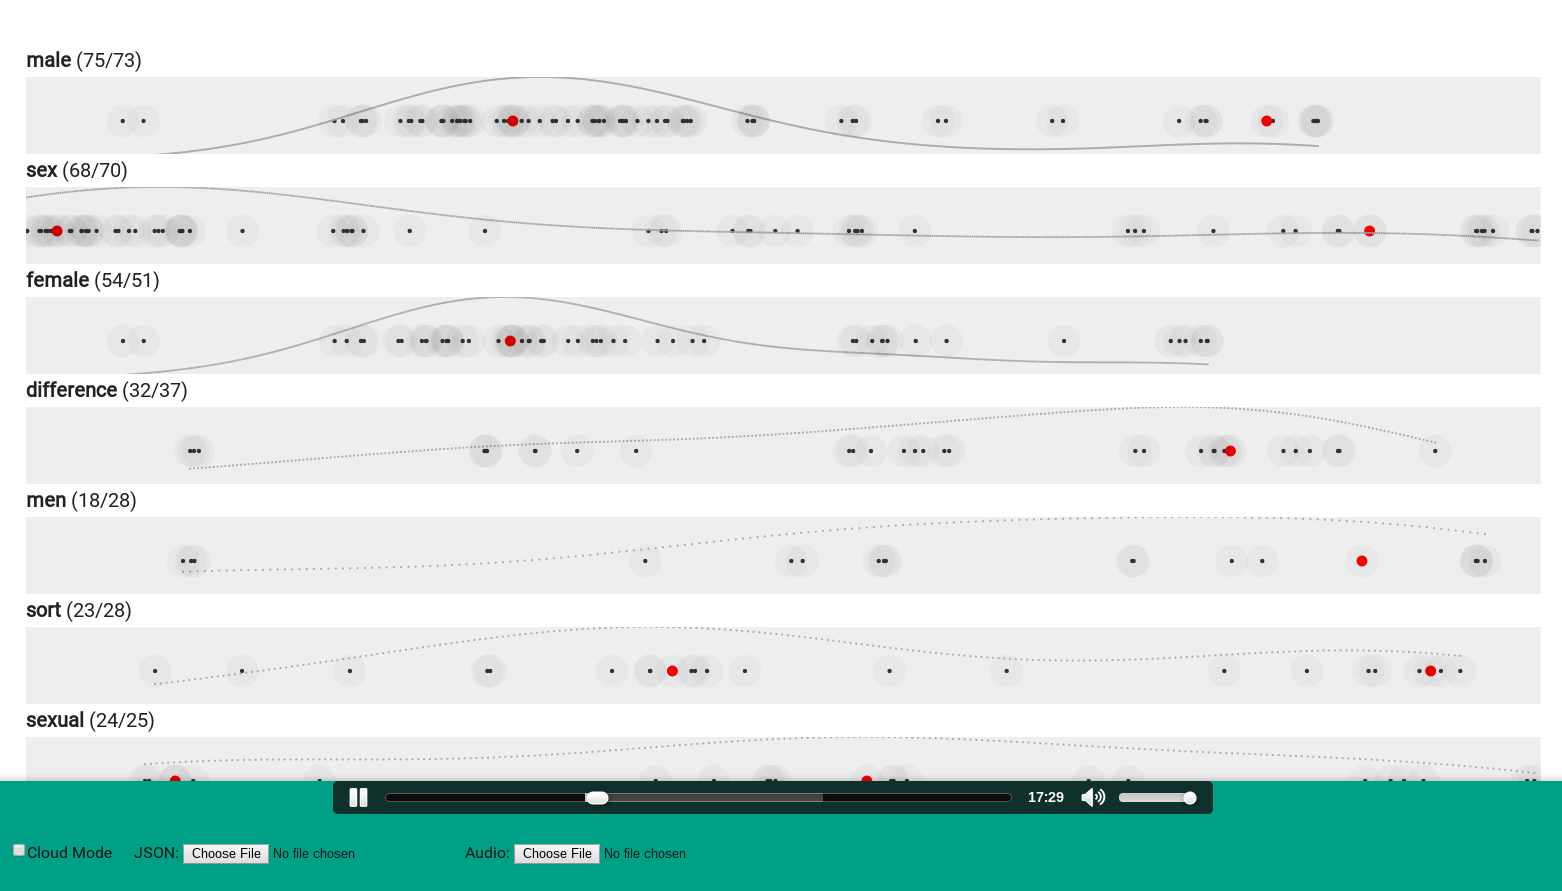
\includegraphics{images/timelines.png}
\caption{Word timelines \label{timelines}}
\end{figure}

The second view (Figure \ref{cloud}) is a \emph{word cloud} with
``semantic axes'', compared to regular word cloud visualizations where
the axes do not have meaning. The x-axis still is the time-axis of the
lecture and the y-axis still is the keyword frequency. The central
feature of this cloud is that it can show \emph{multiple instances} of
one keyword -- one instance for each local maximum. The word instance is
on the same point on the x-axis as the corresponding local maximum. The
timeline for a word can be shown by clicking on it. The example shows
``brain'' in the activated state; the timeline shows up below the cloud.
One can see the two instances of ``brain'' being horizontally aligned
with the two local maxima below\footnote{It is obvious here that the
  first local maximum for the word should rather be at about 30-40\% of
  the word's timeline, but that could be optimized.}. Clicking on the
word also transports the audio to the position of the word next to the
given local maximum. The font size of this word \(W\) is computed by
counting the word occurrences for which holds that the nearest local
maximum is the maximum associated with word \(W\). Additionally multiple
instances of one keyword have the same color to further aid scanning by
allowing the brain to pre-attentively process the representation.

\begin{figure}[htbp]
\centering
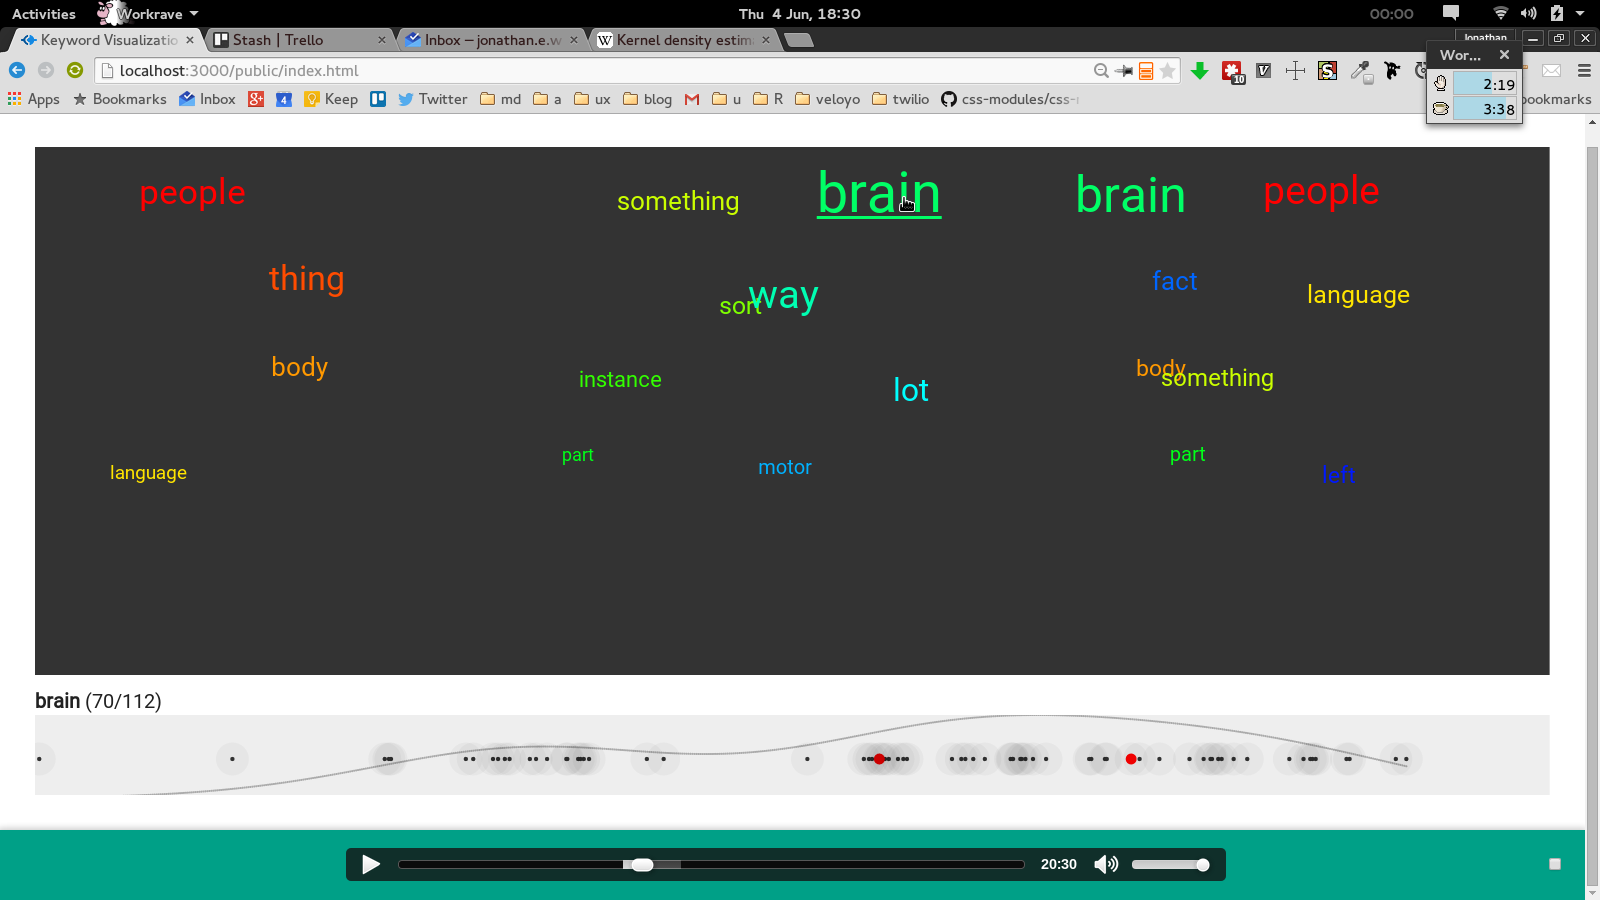
\includegraphics{images/cloud.png}
\caption{Word cloud \label{cloud}}
\end{figure}

This view allows a user to immediately scan the distribution of topics
during the whole lecture. If particularly interested in the parts about
the brain, he/she might click on ``brain'', be immediately transported
to the relevant audio position and additionally have a more in-depth
view in the bottom timeline below the cloud, allowing him/here to
intuitively grasp how long the relevant part might be, maybe flicking
around by clicking on other instances of the word in the timeline.

You could imagine integrating this interface as a semi-transparent
overlay view on a video player, for example on platforms like
lecture2go\footnote{\url{lecture2go.uni-hamburg.de}}, the lecture video
streaming platform used by the University of Hamburg. When using a
system that integrates many lectures in one database like this, it would
also be possible to not only link to keyword instances in the same
lecture but also on a broader scope, e.g the whole course or even other
relevant courses and lectures. Another interesting extension point would
be to integrate human intelligence by allowing to review/score the
quality of keyword instances. This would allow filtering out
false-positives and emphasize the keyword instances that students find
helpful.

\section{Conclusion}\label{conclusion-2}

The primary question of the present thesis was: given that we are
interested in improving speech recognition accuracy of keywords in
university lectures, what is the advantage of creating a
lecture-specific LM and interpolating it with a generic model and how
can we measure this advantage? A secondary question was: how can we use
the results of this approach to provide graphical interfaces for
improving the user's ability to search and scan a given speech medium?

The strategy for answering the primary question consisted in first
explaining the basic concepts of speech recognition and its scientific
history in order to locate our approach in relation to other research
and paradigms. We stated that our approach follows the statistical
pattern-recognition paradigm. This paradigm sees ASR as the process of
measuring features in the acoustic signal and then performing a search
process using these features to find hypotheses using different sources
such as acoustic and language models. Its use of fixed input features
distinguishes it from \emph{integrative approaches} which dynamically
learn the input features.

We furthermore established that lecture transcription can be classified
as \emph{speaker-independent large-vocabulary continuous speech
recognition} (SI-LVCSR).

After explaining the fundamental speech recognition concepts of
phonemes, phonetic dictionaries, search as well as acoustic and language
models, we presented an overview of the scientific work done on lecture
transcription. Here we distinguished generalization and specialization
approaches. While the former try to capture general characteristics of
lectures -- for example by adapting acoustic models to account for
``filler sounds'' which are very common in lectures -- the latter try to
use context specific to a single lecture (\emph{meso} level) or even
parts of a single lecture (\emph{micro} level). Furthermore, methods
using lecture material such as slides can be differentiated into two
groups: those that only use the information existent in the material
itself and those that use ``derived'' data such as Wikipedia articles
crawled by using words from the material as search queries. Our approach
can thus be categorized as a specialization approach operating on the
\emph{meso} level, only using immediately available data for the
material corpus.

In the next step we looked at the 6 lectures from Open Yale Courses that
were used as test data, displaying the heterogenity in quantity and
style of each lecture material. We noted that only 20\% of the available
lectures have lecture material at all, and only 20\% of these have
typical ``slides'', which posed the question if material types such as
excercise sheets or reading assignments have a detrimental effect on the
recognition performance. This however proved not to be the case, as the
later analysis showed.

Our next step was to consider the implementation of the LM-Interpolation
approach. We introduced the general architecture of the \emph{Sphinx 4
Framework} used as the basis for performing speech recognition and
explained the \emph{InterpolatedLanguageModel} component. This component
makes it possible to specify multiple LMs with associated weights in
order to faciliate the interpolation of probabilities for a given
n-gram. We then described the tool pipeline used to perform recognition
and analysis with a baseline and an interpolated run. An important part
in converting the material PDF to a corpus was to ensure that the
conversion result exhibited no superfluous newlines as these would be
represented as sentence boundaries in the resulting material LM, which
would have been an unintended side effect. The intermediate steps and
testcase results are saved in a subfolder of the \texttt{results} folder
of the repository, allowing subsequent inspection of all steps.

This was followed by analyzing the results. The \emph{Keyword Detection
Rate} (KWDR-x) metric was developed to capture the improvement of the
interpolated approach with respect to the formulated research goal of
improving \emph{keyword} recognition. Central modifications to the
canonical \emph{WER} consisted in ignoring word insertions, taking
\emph{lemmas} as the atomic unit and using the material corpus as an
inclusive and the \(top_X\) most common words as an exclusive filter.
The results showed an average improvement in KWDR of 16.8\%, while WER
did not change significantly. This result was compared with the results
of other works. While there is no common metric but the WER to
objectively compare results and WER has the disadvantage of low
relevance to the evaluation goals as discussed above, the overall
impression was that the measured improvement was quite high and at least
serves to validate the usefulness of the explored approach.

Finally we explored the secondary research question of how to make use
of the results for providing graphical interfaces that improve the user
experience when searching and scanning a given speech medium. We noted
that providing a full text display does not make sense for transcription
results with a WER above 30\% as the reading comprehension is too low at
such a rate. An alternative was explored by presenting an interface
prototype that displays a combination of word timelines and a word cloud
with ``semantic axes'', allowing the user to immediately grasp the
overall distribution of keywords during the timeline of a lecture.

\subsection{Improvements and
extensions}\label{improvements-and-extensions}

There are several possible improvements and extensions that were beyond
the scope of the present thesis. The primary one would be to extend the
system to work with different languages. For this thesis, English was
chosen as the only language, primarily because no database with
equivalent test cases like the ones provided by Open Yale Courses was
available for other languages. The combination of quality reference
transcriptions and provided lecture materials is unique, unfortunately.
Also, the manual transcription of a lecture is very time consuming.
Integrating multilinguality into the pipeline would also be no small
task, as preprocessing and lemmatization is language-specific and
suitable equivalent multilanguage tools would have to be found.

As already mentioned above, the approach of filtering out \(top_X\)
words could possibly be solved more elegantly by using \emph{tf/idf} to
compute ``keyword-ness'' of words; this would help eliminate the cases
where keywords that are part of the \(top_X\) words are filtered out.

More extensive empirical evaluation should be performed on the
interpolation weights in order to achieve reliable results concerning
the relationship of weights to \(\Delta KWDR\) and \(\Delta WER\). While
this has not been the primary focus of our evaluation, it is of
importance for applications, as they could choose a weighting according
to their focus on sentence integrity: an application not displaying full
text would likely choose a high value for the material corpus' weight;
accordingly an application actually showing full text would likely
choose a weighting which does at least not diminish general recognition
performance.

\section*{References}\label{references}
\addcontentsline{toc}{section}{References}

\hyperdef{}{ref-cettolo}{\label{ref-cettolo}}
Cettolo, M., Brugnara, F., \& Federico, M. (2004). Advances in the
automatic transcription of lectures. In \emph{Acoustics, speech, and
signal processing, 2004. proceedings.(ICASSP'04). iEEE international
conference on} (Vol. 1, pp. I--769). IEEE.

\hyperdef{}{ref-cmuDict}{\label{ref-cmuDict}}
\emph{cmudict-en-us.dict}. (2015).
\url{https://github.com/cmusphinx/sphinx4/blob/master/sphinx4-data/src/main/resources/edu/cmu/sphinx/models/en-us/cmudict-en-us.dict}.

\hyperdef{}{ref-cmuLm}{\label{ref-cmuLm}}
\emph{cmusphinx-5.0-en-us.lm}. (2015).
\url{http://sourceforge.net/projects/cmusphinx/files/Acoustic\%20and\%20Language\%20Models/US\%20English\%20Generic\%20Language\%20Model/}.

\hyperdef{}{ref-cruttenden2014gimson}{\label{ref-cruttenden2014gimson}}
Cruttenden, A. (2014). \emph{Gimson's pronunciation of English}.
Routledge.

\hyperdef{}{ref-florian1996blackwell}{\label{ref-florian1996blackwell}}
Florian, C. (1996). The Blackwell encyclopedia of writing systems.
\emph{Oxford: Blackwell}.

\hyperdef{}{ref-glass}{\label{ref-glass}}
Glass, J., Hazen, T. J., Hetherington, L., \& Wang, C. (2004). Analysis
and processing of lecture audio data: Preliminary investigations. In
\emph{Proceedings of the workshop on interdisciplinary approaches to
speech indexing and retrieval at hLT-nAACL 2004} (pp. 9--12).
Association for Computational Linguistics.

\hyperdef{}{ref-hinton2012deep}{\label{ref-hinton2012deep}}
Hinton, G., Deng, L., Yu, D., Dahl, G. E., Mohamed, A.-r., Jaitly, N.,
Senior, A., et al. (2012). Deep neural networks for acoustic modeling in
speech recognition: The shared views of four research groups.
\emph{Signal Processing Magazine, IEEE}, \emph{29}(6), 82--97. IEEE.

\hyperdef{}{ref-kato2000}{\label{ref-kato2000}}
Kato, K., Nanjo, H., \& Kawahara, T. (2000). Automatic transcription of
lecture speech using topic-independent language modeling. In \emph{Sixth
international conference on spoken language processing}.

\hyperdef{}{ref-kawahara08}{\label{ref-kawahara08}}
Kawahara, T., Nemoto, Y., \& Akita, Y. (2008). Automatic lecture
transcription by exploiting presentation slide information for language
model adaptation. In \emph{Acoustics, speech and signal processing,
2008. iCASSP 2008. iEEE international conference on} (pp. 4929--4932).
IEEE.

\hyperdef{}{ref-lai}{\label{ref-lai}}
Lai, J., Karat, C.-M., \& Yankelovich, N. (2008). Conversational speech
interfaces and technologies. \emph{The human-computer interaction
handbook: Fundamentals, evolving technologies and emerging
applications}, 481--491.

\hyperdef{}{ref-marquard}{\label{ref-marquard}}
Marquard, S. (2012). Improving searchability of automatically
transcribed lectures through dynamic language modelling. University of
Cape Town.

\hyperdef{}{ref-miranda}{\label{ref-miranda}}
Miranda, J., Neto, J. P., \& Black, A. W. (2013). Improving aSR by
integrating lecture audio and slides. In \emph{Acoustics, speech and
signal processing (iCASSP), 2013 iEEE international conference on} (pp.
8131--8135). IEEE.

\hyperdef{}{ref-munteanu}{\label{ref-munteanu}}
Munteanu, C., Penn, G., \& Baecker, R. (2007). Web-based language
modelling for automatic lecture transcription. In \emph{INTERSPEECH}
(pp. 2353--2356).

\hyperdef{}{ref-rabiner}{\label{ref-rabiner}}
Rabiner, L., \& Juang, B.-H. (1993). Fundamentals of speech recognition.
Prentice hall.

\hyperdef{}{ref-whitepaper}{\label{ref-whitepaper}}
Walker, W., Lamere, P., Kwok, P., Raj, B., Singh, R., Gouvea, E., Wolf,
P., et al. (2004). Sphinx-4: A flexible open source framework for speech
recognition. Sun Microsystems, Inc.

\hyperdef{}{ref-yamazaki}{\label{ref-yamazaki}}
Yamazaki, H., Iwano, K., Shinoda, K., Furui, S., \& Yokota, H. (2007).
Dynamic language model adaptation using presentation slides for lecture
speech recognition. \emph{Proc. INTERSPEECH 2007}, 2349--2352.

\newpage
\thispagestyle{empty}
\section*{Eidesstattliche Erklärung} 

Ich versichere, dass ich die vorstehende Arbeit selbstständig und ohne fremde Hilfe angefertigt und mich anderer als der im beigefügten Verzeichnis angegebenen Hilfsmittel nicht bedient habe. Alle Stellen, die wörtlich oder sinngemäß aus Veröffentlichungen entnommen wurden, sind als solche kenntlich gemacht. \\

%\noindent Ich bin mit einer Einstellung in den Bestand der Bibliothek des Fachbereiches einverstanden.

\vspace{2cm}

\noindent Hamburg, den \uline{~~~~~~~~~~~~~~~~~~~~}~~~~~Unterschrift: \uline{~~~~~~~~~~~~~~~~~~~~~~~~~~~~~~~~~~~~~~~~~~~~~~~~~~}

\end{document}
